\documentclass[10pt]{book}
\usepackage{mybookstyle}
\settheme{green}
%%%%%%%%%%%%%%%%%%%%%%%%%%%%%%
% LỆNH CUSTOM
%%%%%%%%%%%%%%%%%%%%%%%%%%%%%%
\newcommand{\tamgiac}{\triangle}
\newcommand{\dg}{^\circ}
\newcommand{\tuongduong}{\Leftrightarrow}
\newcommand{\suyra}{\Rightarrow}
\newcommand{\goc}{\widehat}
\newcommand{\vuong}{\perp}
\newcommand{\thuoc}{\in}
\newcommand{\khac}{\ne}
\newcommand{\dongdang}{\sim}
\newcommand{\can}{\sqrt}
\newcommand{\R}{\mathbb{R}}
\newcommand{\Q}{\mathbb{Q}}
\newcommand{\I}{\mathbb{I}}
\newcommand{\Z}{\mathbb{Z}}
\newcommand{\N}{\mathbb{N}}
\newcommand{\xd}{\\[0.5em]}
\newcommand{\xdd}{\par\vspace{6pt}}
\newcommand{\nn}[1]{\left\{ #1 \right\}}
\newcommand{\nv}[1]{\left[ #1 \right]}  
\newcommand{\nt}[1]{\left( #1 \right)}
\newcommand{\va}{\wedge}
\newcommand{\hoac}{\vee}


\newcommand{\cung}[1]{%
	\begin{tikzpicture}[baseline=(cung.base)]
		\node[inner sep=0,text height=1ex,text depth=0.2ex] (cung) at (0,0) {$\textit{#1}$};
		\draw[line width=0.5pt] ([xshift=0.2em, yshift=0.3em]cung.north west) to[out=45,in=135] ([xshift=0.2em, yshift=0.3em]cung.north east);
	\end{tikzpicture}
}
%\usepackage{showframe}

\begin{document}
%===== MỤC LỤC =====%
\newgeometry{
  left=35pt,
  top=2.5cm,
  bottom=2.5cm,
  bindingoffset=0.8cm
}
\tableofcontents
\clearpage
\restoregeometry
%===== MỤC LỤC =====%

%===== NỘI DUNG =====%

%----- CHƯƠNG 1 -----%
\setchapterabstract{Chuyên đề đi sâu vào giải quyết các dạng bài tập liên quan đến phương trình bậc 2 như: Giải phương trình bậc hai, vẽ đồ thị, định lý vi-et,...}
\chapter{PHƯƠNG TRÌNH BẬC 2}
\chaptoc[0.75cm]


\section{Giải phương trình bậc 2}
\subsection{Phương trình bậc 2}
%-----Định nghĩa-----%
\dn{Phương trình bậc 2}{
\textbullet Phương trình bậc 2 có dạng: $ax^2 + bx + c = 0~(a \khac 0)$\mn[-2\baselineskip]{$a \khac 0$ là một điều kiện quan trọng để phương trình trên là phương trình bậc 2 \xd Nếu $a = 0$ \xd $\suyra 0x^2 + bx + c = 0$ \xd $\suyra bx + c = 0$~(Đây là phương trình bậc 1)} $(b,c \thuoc \R)$\mn[4.5\baselineskip]{$b,c \thuoc \R$ nghĩa là 2 số $b, c$ có thể là bất cứ số nào.}.
}
\ex{Phương trình bậc 2}{
    1. $2x^2 = 0$ \xd
    2. $-x^2 + 2x +8 =0$ \xd
    3. $x^2 -9 = 0$
}
\subsection{Phương pháp giải phương trình bậc 2}
\ex{Giải bằng cách sử dụng \textit{hằng đẳng thức}}{
\[ 
\colorbox{themecolor!10!white}{$2x^2 - 5x + 2 = 0$} 
\]
\textbullet\; Bước 1: Chia cả 2 vế cho $a = 2$.  
\[
\frac{2x^2}{2} - \frac{5x}{2} + \frac{2}{2} = \frac{0}{2}
\]
\[
\suyra\; \colorbox{themecolor!10!white}{$x^2 - \frac{5}{2}x + 1 = 0$}
\]
\textbullet\; Bước 2: Biến đổi phương trình trên thành 1 trong 2 hằng đẳng thức là:
\[
\begin{cases}
 A^2 +2AB + B^2 = (A+B)^2 \xd
 A^2 -2AB + B^2 = (A-B)^2
\end{cases}
\]
\[
\suyra \nv{x^2 - 2 \cdot x \cdot \frac{5}{4} + \nt{\frac{5}{4}}^2} - \nt{\frac{5}{4}}^2 +1 = 0
\]
\mn[-5\baselineskip]{$\frac{5}{4} = -\frac{5}{2} : (-2)$} \mn[-3\baselineskip]{Cộng thêm $\nt{\frac{5}{4}}^2$ thì trừ đi $\nt{\frac{5}{4}}^2$ để không làm thay đổi đề bài}
\[
\suyra \nt{x-\frac{5}{4}}^2 - \nt{\frac{5}{4}}^2 +1 = 0
\]
\[
\suyra \nt{x-\frac{5}{4}}^2 - \frac{9}{16} = 0
\]
\[
\suyra \nt{x-\frac{5}{4}}^2 - \nt{\frac{3}{4}}^2 = 0
\]
\mn[-1\baselineskip]{Ta có thể tìm $\nt{\frac{3}{4}}$ bằng cách $\can{\frac{9}{16}}$}
\[
\suyra \nt{x-\frac{5}{4}-\frac{3}{4}}\nt{x-\frac{5}{4}+\frac{3}{4}} = 0
\]
\[
\suyra (x-2)\nt{x-\frac{1}{2}} = 0
\]
\[
\suyra x-2 = 0 ~\hoac~ x-\frac{1}{2} = 0
\]
\[
\suyra x = 2 ~\hoac~ x=\frac{1}{2}
\]
}
\ex{Giải bằng cách sử dụng biệt thức}{
\[ 
\colorbox{themecolor!10!white}{$2x^2 - 5x + 2 = 0$} 
\]
\textbullet Bước 1: Tính biệt thức $\Delta$
\[
\Delta = b^2 -4ac = (-5)^2 - 4.2.2 = 9
\]
\textbullet Bước 2: Nhận xét \xd
Nếu $\Delta < 0 \suyra$ Phương trình vô nghiệm \xd
Nếu $\Delta = 0 \suyra$ Phương trình có nghiệm kép (2 nghiệm giống nhau) $\suyra x = \frac{-b}{2a}$ \xd
Nếu $\Delta > 0 \suyra$ Phương trình có 2 nghiệm phân biệt (2 nghiệm khác nhau)
\[
    x = \frac{-b + \can{\Delta}}{2a} ~ \hoac ~ x = \frac{-b - \can{\Delta}}{2a}
\]
Ta có: \[ \Delta = 9 > 0 \suyra \text{Phương trình có 2 nghiệm phân biệt}\] 
\[
\suyra x = \frac{-(-5) + \can{9}}{2.2} ~ \hoac ~ x = \frac{-(-5) - \can{9}}{2.2}
\]
\[
\suyra x = 2 ~ \hoac ~ x = \frac{1}{2}
\]
}

\section{Đồ thị hàm số}
\dn{Đồ thị hàm số bậc 2}{
    \textbullet Trong chương trình học ta chỉ khảo sát hàm số bậc 2 có dạng $y=ax^2$ \xd 
    $(a \khac 0)$. \xd 
    \textbullet Hàm số bậc 2 nói chung đều có dạng một đường cong gọi là \textit{Parabol}. \xd 
    \textbullet Đường cong Parabol có hai loại: Úp lên ($a > 0$) hoặc úp xuống ($ a < 0$).
    }

  \begin{figure}[h]
		\subfloat[$(a > 0)$\label{hinh1a}]{\includegraphics[width=0.35\textwidth]{img/Do_thi_ham_so_bac_2a.pdf}}\hfill
		\subfloat[$(a < 0)$\label{hinh1b}]{\includegraphics[width=0.35\textwidth]{img/Do_thi_ham_so_bac_2b.pdf}}
		\caption{2 hình dạng Parabol}
		\label{hinh1.1}
\end{figure}

\subsection{Cách vẽ Parabol}
\ex{Cách vẽ Parabol}{
  Vẽ đồ thị hàm số: 
  \[
    \colorbox{themecolor!10!white}{$y = x^2$}
  \]
  Bước 1: Lập bảng giá trị \xd 
  	\begin{tabularx}{\textwidth}{CCCCCC}
    \arrayrulecolor{themecolor!40!white}
		\midrule
		$x$     & $-2$ & $-1$ & $0$ & $1$ & $2$ \\
    $y=x^2$ &  $4$ & $1$  & $0$ & $1$ & $4$ \\
    \midrule
	  \end{tabularx}
    \mn[-3.5\baselineskip]{
      Một số quy tắc khi lập bảng: \xd
      \textbullet Chọn các giá trị $x$ có tính đối xứng. \xd
      \textbullet Chọn các giá trị $x$ mà cho ra một kết quả $y$ dễ dàng vẽ.
       }

  Bước 2: Vẽ trục tọa độ $Oxy$
    \begin{center}
      \includegraphics[width=0.5\textwidth]{img/Truc_Oxy.pdf}
      \captionsetup{hypcap=false}
      \captionof{figure}{Trục $Oxy$}
      \label{hinh1.2}
    \end{center}
      \mn[-12\baselineskip]{
        Một số lưu ý khi vẽ trục: \xd 
        \textbullet Chỉ vẽ vừa đủ các giá trị, không vẽ quá nhiều giá trị không có trong bảng. \xd
        \textbullet Kích cỡ số vừa đủ, không vẽ quá to, để tốt hơn về mặt thị giác.
      }

  Bước 3: Vẽ các điểm có trong bảng lên trục $Oxy$ \xd
    \begin{center}
      \includegraphics[width=0.5\textwidth]{img/Truc_Oxy_co_diem.pdf}
      \captionsetup{hypcap=false}
      \captionof{figure}{Các điểm trên trục $Oxy$}
      \label{hinh1.3}
    \end{center}

  Bước 4: Sử dụng thước Parabol để vẽ
    \begin{center}
		  \includegraphics[width=0.3\textwidth]{img/Parabol_trai.pdf}\hfill
		  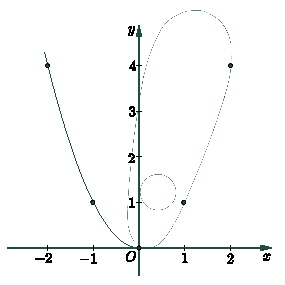
\includegraphics[width=0.3\textwidth]{img/Parabol_phai.pdf}\hfill
      \includegraphics[width=0.3\textwidth]{img/Parabol_full.pdf}
      \captionsetup{hypcap=false}
		  \captionof{figure}{Cách dùng thước Parabol để vẽ}
		  \label{hinh1.4}
    \end{center}
    \mn[-11.5\baselineskip]{
      Một số lưu ý khi sử dụng Parabol: \xd 
      \textbullet Parabol có hai đầu, ta lựa chọn 1 trong 2 đầu để vẽ. \xd 
      \textbullet Đỉnh của Parabol có xu hướng bị nhọn, điều này là bình thường do cấu tạo của thước, có thể sử dụng tay để đồ nhẹ lại đỉnh để tạo cảm giác cong. \xd 
      \textbullet Đỉnh của Parabol nếu quá nhọn sẽ bị trừ điểm.
      }    
}

\newpage
\section{Định lý Viète}
François Viète (1540 – 1603) là một nhà toán học người Pháp, thường được xem là “cha đẻ của đại số hiện đại”. Ông sinh tại Fontenay-le-Comte (Pháp) trong một gia đình luật sư, và bản thân cũng từng học luật trước khi chuyển hướng nghiên cứu toán học. Viète nổi bật với việc đưa ra cách dùng chữ cái để biểu diễn các ẩn và hệ số trong phương trình, đặt nền móng cho ký hiệu đại số ngày nay.
\xdd 
Ngoài sự nghiệp toán học, Viète còn là cố vấn pháp lý và từng phục vụ trong triều đình của vua Henry IV. Các công trình của ông không chỉ giúp giải quyết nhiều bài toán khó thời bấy giờ mà còn ảnh hưởng sâu rộng đến sự phát triển của toán học châu Âu. Định lý Viète về mối quan hệ giữa nghiệm và hệ số của phương trình bậc hai đến nay vẫn được giảng dạy trong chương trình phổ thông.

\begin{marginfigure}|-4.5cm|
	\centering
	\includegraphics[width=0.65\marginparwidth]{img/Francois_Viete.jpg}
	\vspace{0.5cm}
	\margincaption{François Viète (1540 – 1603)}
	\label{hinh1.5}
\end{marginfigure}

\subsection{Tổng quan định lý Viète}
\thm{Viète}{
    Nếu phương trình bậc 2: $ax^2 + bx + c = 0$ có nghiệm (nghiệm kép hoặc 2 nghiệm phân biệt) thì: \xd 
    \[
        S = x_1 + x_2 = \frac{-b}{a}
    \]

    \[
        P = x_1.x_2 = \frac{c}{a}
    \]

    \textit{Định lý Viète cho phép biết mối quan hệ giữa tổng và tích của 2 nghiệm với hệ số mà không cần phải tính 2 nghiệm chính xác.}
}

    Kiểm chứng định lý Viète thông qua ví dụ sau:
    \ex{Viète}{
        Xét phương trình sau:
        \[
            \colorbox{themecolor!10!white}{$x^2 -5x +6 = 0$}  
        \]

        \[
            \Delta = b^2 - 4ac = (-5)^2 - 4.1.6 = 1 > 0
        \]

        Vậy phương trình có 2 nghiệm phân biệt.

        \[
            S = x_1 + x_2 = \frac{-b}{a} = \frac{5}{1} = 5
        \]

        \[
            P = x_1.x_2 = \frac{c}{a} = \frac{6}{1} = 6
        \]

        Tính nghiệm trực tiếp:
        \[
            x_1 = \frac{-b + \can{\Delta}}{2a} ~\hoac~ x_2 = \frac{-b-\can{\Delta}}{2a}
        \]

        \[
            x_1 = \frac{--5 + \can{1}}{2.1} = 3 ~\hoac~ x_2 = \frac{--5-\can{1}}{2} = 2
        \]

        \[
            x_1 + x_2 = 3 + 2 = 5 \text{~và~} x_1.x_2 = 3.2 = 6
        \]

        Vậy định lý Viète là đúng.
    }
\newpage
\subsection{Tìm 2 số khi biết tổng và tích của chúng}
\hq{
    Nếu hai số có tổng và tích lần lượt bằng $S$ và $P$ thì hai số đó là nghiệm của phương trình: 
    \[
        x^2 - Sx + P = 0~~(S^2 -4P \geq  0)
    \]
}{
\xdd     
Giả sử: $x_1$ hoặc $x_2$ là 2 nghiệm của phương trình bậc hai bất kì.\xd 
Ta có: $S = x_1 + x_2$ và $P = x_1.x_2$ \xd 
Theo hệ quả $x_1$ hoặc $x_2$ là hai nghiệm của phương trình:
\[
    x^2 - Sx + P = 0
\]
\[
    \suyra x^2 -(x_1+x_2)x +x_1.x_2 = 0
\]
\[
    \suyra x^2 - x_1.x - x_2.x +x_1.x_2 = 0
\]
\[
    \suyra x(x - x_1) - x_2(x - x_1) = 0
\]
\[
    \suyra (x - x_1)(x - x_2) = 0
\]
\[
    \suyra x - x_1 = 0 ~\hoac~ x - x_2 = 0 
\]
\[
    \colorbox{themecolor!10!white}{$\suyra x = x_1 ~\hoac~ x = x_2$}
\]
}

\ex{Tìm 2 số khi biết tổng và tích của chúng lần lượt là 7 và 10}{
    Hai số đó sẽ là nghiệm của phương trình:
    \[
        \colorbox{themecolor!10!white}{$x^2 -7x + 10 = 0$}
    \]
    \[
        \Delta = S^2 - 4P = (-7)^2 -4.10 = 9 > 0
    \]
    Phương trình có 2 nghiệm phân biệt: \xd 
    \[
        x_1 = \frac{7 + \can{9}}{2} = 5 ~\hoac~ x_2 = \frac{7 - \can{9}}{2} = 2
    \]
    Vậy 2 số đó là 7 hoặc 10.
}

\subsection{Nhẩm nghiệm của phương trình bậc 2}

\noindent\textbullet Nếu phương trình $ax^2 + bx + c = 0~(a \khac 0)$ có $a + b + c = 0$ thì phương trình có nghiệm là: $x_1 = 1;~ x_2 = \frac{c}{a}$ \xd 
\textbullet Nếu phương trình $ax^2 + bx + c = 0~(a \khac 0)$ có $a - b + c = 0$ thì phương trình có nghiệm là: $x_1 = -1;~ x_2 = -\frac{c}{a}$

\ex{không giải mà nhẩm nghiệm của phương trình sau:}{
    \[
        \colorbox{themecolor!10!white}{$15x^2 +7x - 22 = 0$}
    \]
    Có: $a + b + c = 15 + 7 + (-22) = 0$ \xd 
    Vậy phương trình có hai nghiệm là: $x_1 = 1;~ x_2 = \frac{c}{a} = \frac{-22}{15}.$
}

\baitap
\vspace{-1cm}
\subsection{Dạng 1: Giải phương trình bậc 2}
\vspace{0.5cm}
\begin{smallfont}
%-----Bài 1-----%
    \bt[CTST Tập 2 Tr.14]{
    Giải các phương trình sau: 
	\begin{multicols}{2}
    \begin{enumerate}[label=\alph*)]
		\item 
		$7x^2 -3x + 2 = 0$
		\item 
		$3x^2 - 2\can{3}x + 1 = 0$
        \item 
        $-2x^2 + 5x +2 = 0$
        \item 
        $5x^2 -12x + 4 = 0$
        \item 
        $5x^2 -2\can{5}x + 1 = 0$
        \item 
        $x^2 -x -20 = 0$
        \item 
        $6x^2 -11x -35 =0$
        \item 
        $16y^2 +24y +9 =0$
	\end{enumerate}
    \end{multicols}
    \textbf{\textit{Gợi ý:}}
    \begin{multicols}{2}
    \begin{enumerate}[label=\alph*)]
		\item 
		$\Delta = -47$
		\item 
        $\Delta = 0$
		\item 
        $\Delta = 41$
        \item 
        $\Delta = 64$
		\item 
        $\Delta = 0$
        \item 
        $\Delta = 81$
        \item 
        $\Delta = 961$
        \item 
        $\Delta = 0$
	\end{enumerate}
    \end{multicols}
    }

\end{smallfont}
\vspace{0.5cm}
\subsection{Dạng 2: Vẽ đồ thị Parabol và phương trình hoành độ giao điểm}
\vspace{0.5cm}
\begin{smallfont}
    %-----Bài 1-----%
    \bt[TUYỂN SINH TP.HCM 2018-2019]{
        Cho Parabol $(P): y=x^2$ và đường thẳng $(d): y=3x-2$.
        \begin{enumerate}[label=\alph*)]
            \item 
            Vẽ $(P)$ và $(d)$ trên cùng hệ trục tọa độ.
            \item 
            Tìm tọa độ giao điểm của $(P)$ và $(d)$ bằng phép tính.
        \end{enumerate}
    }
    \xdd 
    %-----Bài 2-----%
    \bt[TUYỂN SINH TP.HCM 2019-2020]{
        Cho Parabol $(P): y=-\frac{1}{2}x^2$ và đường thẳng $(d): y=x-4$.
        \begin{enumerate}[label=\alph*)]
            \item 
            Vẽ $(P)$ và $(d)$ trên cùng hệ trục tọa độ.
            \item 
            Tìm tọa độ giao điểm của $(P)$ và $(d)$ bằng phép tính.
        \end{enumerate}
    }
    \xdd 
    %-----Bài 3-----%
    \bt[TUYỂN SINH TP.HCM 2020-2021]{
        Cho Parabol $(P): y=\frac{1}{4}x^2$ và đường thẳng $(d): y=-\frac{1}{2}x+2$.
        \begin{enumerate}[label=\alph*)]
            \item 
            Vẽ $(P)$ và $(d)$ trên cùng hệ trục tọa độ.
            \item 
            Tìm tọa độ giao điểm của $(P)$ và $(d)$ bằng phép tính.
        \end{enumerate}
    }
    \xdd 
    %-----Bài 4-----%
    \bt[TUYỂN SINH TP.HCM 2022-2023]{
        Cho Parabol $(P): y=x^2$ và đường thẳng $(d): y=-x+2$.
        \begin{enumerate}[label=\alph*)]
            \item 
            Vẽ $(P)$ và $(d)$ trên cùng hệ trục tọa độ.
            \item 
            Tìm tọa độ giao điểm của $(P)$ và $(d)$ bằng phép tính.
        \end{enumerate}
    }
    \xdd 
    %-----Bài 5-----%
    \bt[TUYỂN SINH TP.HCM 2023-2024]{
        Cho Parabol $(P): y=\frac{x^2}{2}$ và đường thẳng $(d): y=x+4$.
        \begin{enumerate}[label=\alph*)]
            \item 
            Vẽ $(P)$ và $(d)$ trên cùng hệ trục tọa độ.
            \item 
            Tìm tọa độ giao điểm của $(P)$ và $(d)$ bằng phép tính.
        \end{enumerate}
    }
    \xdd 
    %-----Bài 6-----%
    \bt[TUYỂN SINH TP.HCM 2024-2025]{
        Cho Parabol $(P): y=\frac{x^2}{2}$.
        \begin{enumerate}[label=\alph*)]
            \item 
            Vẽ $(P)$ trên hệ trục tọa độ.
            \item 
            Tìm tọa độ các điểm thuộc $(P)$ có tung độ bằng 18.
        \end{enumerate}
        \xdd 
        \textbf{\textit{Gợi ý:}}
        \xdd 
        \textbullet  Tung độ bằng 18 $\suyra y = 18$.
    }
    \xdd 
    %-----Bài 7-----%
    \bt[TUYỂN SINH SÓC TRĂNG 2024-2025]{
        Cho hàm số $y=x^2$ có đồ thị $(P)$
        \begin{enumerate}[label=\alph*)]
            \item 
            Vẽ đồ thị $(P)$ trên mặt phẳng tọa độ $Oxy$.
            \item 
            Trên mặt phẳng tọa độ $Oxy$, xét điểm $A$ có hoành độ bằng 5 và $A$ nằm trên đường thẳng $(d): y=3x+1$. Tìm tọa độ các điểm nằm trên đồ thị $(P)$ có cùng tung độ với điểm $A$.
        \end{enumerate}
        \xdd 
        \textbf{\textit{Gợi ý:}}
        \xdd
        \textbullet  Đề yêu cầu: "Tìm tọa độ các điểm nằm trên đồ thị $(P)$ có cùng tung độ với điểm $A$". \xd 
        $\suyra$ Tìm tung độ điểm $A$. \xd 
        \textbullet Điểm $A$ có hoành độ bằng 5 và $A$ nằm trên đường thẳng $(d): y=3x+1$. \xd 
        $\suyra$ đường thẳng $(d): y=3x+1$ đi qua điểm $A(5; y_A)$. \xd 
        $\suyra$ thay điểm $A$ vào $(d)$ để tìm tung độ điểm $A$ hay $(y_A)$.
        
    }
    \xdd 
    %-----Bài 8-----%
    \bt[TUYỂN SINH TRÀ VINH 2024-2025]{
        Trong mặt phẳng tọa độ $Oxy$, Cho Parabol $(P): y=2x^2$ và đường thẳng $(d):y=-2x+4$.
        \begin{enumerate}[label=\alph*)]
            \item 
            Vẽ đồ thị hai hàm số $(P)$ và $(d)$.
            \item 
            Bằng phép toán tìm tọa độ giao điểm của $(P)$ và $(d)$.
        \end{enumerate}
    }
    \xdd 
    %-----Bài 9-----%
    \bt[TUYỂN SINH TIỀN GIANG 2024-2025]{
        Trong mặt phẳng tọa độ $Oxy$, Cho Parabol $(P): y=2x^2$.
        \begin{enumerate}[label=\alph*)]
            \item 
            Vẽ đồ thị hàm số $(P)$.
            \item 
            Bằng phép toán hãy tìm các điểm thuộc $(P)$ có tung độ bằng 14.
        \end{enumerate}
        \xdd 
        \textbf{\textit{Gợi ý:}}
        \xdd 
        \textbullet  Tung độ bằng 14 $\suyra y = 14$.
    }
    \xdd 
    %-----Bài 10-----%
    \bt[TUYỂN SINH AN GIANG 2024-2025]{
        Cho hàm số $y=-0,5x^2$
        \begin{enumerate}[label=\alph*)]
            \item 
            Vẽ đồ thị hàm số trên hệ trục $Oxy$.
            \item 
            Tìm các điểm thuộc đồ thị hàm số đã cho có tung độ bằng $-18$.
        \end{enumerate}
        \xdd 
        \textbf{\textit{Gợi ý:}}
        \xdd 
        \textbullet  Tung độ bằng $-18$ $\suyra y = -18$.
    }
    \xdd 
    %-----Bài 11-----%
    \bt[TUYỂN SINH NINH THUẬN 2025-2026]{
        Cho hàm số $y=2x^2$ có đồ thị $(P)$.
        \begin{enumerate}[label=\alph*)]
            \item 
            Vẽ đồ thị $(P)$ của hàm số.
            \item 
            Tìm các điểm thuộc Parabol $(P)$ có tung độ bằng 2.
        \end{enumerate}
        \xdd 
        \textbf{\textit{Gợi ý:}}
        \xdd 
        \textbullet  Tung độ bằng 2 $\suyra y = 2$.
    }
    \xdd 
    %-----Bài 12-----%
    \bt[TUYỂN SINH ĐÀ NẴNG 2025-2026]{
        Cho hàm số $y=-\frac{1}{2}x^2$ có đồ thị $(P)$.
        \begin{enumerate}[label=\alph*)]
            \item 
            Vẽ đồ thị $(P)$ của hàm số.
            \item 
            Tìm các điểm thuộc Parabol $(P)$ có tung độ bằng 5 lần hoành độ.
        \end{enumerate}
        \xdd 
        \textbf{\textit{Gợi ý:}}
        \xdd 
        \textbullet  Tung độ bằng 5 lần hoành độ. \xd 
        $\suyra y = 5x$.
    }
    \xdd 
    %-----Bài 13-----%
    \bt{
        Cho hàm số $y=\frac{1}{4}x^2$ có đồ thị $(P)$ và đường thẳng $(d): y=\frac{1}{2}x + 2$.
        \begin{enumerate}[label=\alph*)]
            \item 
            Vẽ $(P)$ và $(d)$ trên cùng một hệ trục tọa độ.
            \item 
            Tìm tọa độ giao điểm của $(P)$ và $(d)$ bằng phép tính.
            \item 
            Tìm phương trình đường thẳng $(d')$ song song với $(d)$ và cắt $(P)$ tại điểm có hoành độ là 2.
        \end{enumerate}
        \xdd 
        \textbf{\textit{Gợi ý:}}
        \xdd 
        \textbullet Phương trình đường thẳng $(d')$ có dạng $y = ax + b$. \xd 
        \textbullet $(d')$ song song với $(d)$ $\suyra a =\frac{1}{2}$ 
        $\suyra y = \frac{1}{2}x + b$. \xd
        \textbullet  $(d')$ cắt $(P)$ tại điểm có hoành độ là 2. \xd 
        $\suyra$ Phương trình hoành độ giao điểm giữa $(P)$ và $(d')$ có nghiệm là $x=2$.
    }
    \xdd 
    %-----Bài 14-----%
    \bt[TUYỂN SINH QUẢNG NAM 2024-2025]{
        Trên mặt phẳng tọa độ $Oxy$, cho đường thẳng $(d): y = ax + b$. Tìm các hệ số $a, b$ biết $(d)$ có hệ số góc bằng $-2$ và $(d)$ cắt Parabol $(P): y = \frac{2}{3}x^2$ tại điểm $M$ có hoành độ dương và tung độ bằng 6.
        \xdd 
        \textbf{\textit{Gợi ý:}}
        \xdd 
        $(d)$ có hệ số góc bằng $-2 \suyra a = -2$ \xd 
        $(d)$ cắt Parabol $(P): y = \frac{2}{3}x^2$ tại điểm $M$ có hoành độ dương và tung độ bằng 6. \xd 
        $\suyra (d)$ cắt Parabol $(P): y = \frac{2}{3}x^2$ tại điểm $M(x_M ; 6)~(x_M > 0)$ \xd 
        $\suyra$ Phương trình hoành độ giao điểm giữa $(P)$ và $(d)$ có nghiệm $x_M > 0$ \xd 
        }
    \xdd 
    %-----Bài 15-----%
    \bt[THI THỬ TRƯỜNG TRẦN QUỐC TOẢN 1 THỦ ĐỨC]{
        \begin{enumerate}[label=\alph*)]
            \item 
            Vẽ đồ thị $(P)$ của hàm số $y=\frac{x^2}{2}$.
            \item 
            Tìm những điểm $A$ thuộc $(P)$ có tung độ gấp đôi hoành độ.
        \end{enumerate}
        \xdd 
        \textbf{\textit{Gợi ý:}}
        \xdd
        \textbullet  Tung độ gấp đôi hoành độ. \xd 
        $\suyra y = 2x$
    }
    \xdd 
    %-----Bài 16-----%
    \bt[THI THỬ TRƯỜNG HỒNG BÀNG TP.HCM 2025-2026]{
    Cho Parabol $(P): y =\frac{x^2}{4}$
    \begin{enumerate}[label=\alph*)]
            \item 
            Vẽ $(P)$ trên hệ trục $Oxy$.
            \item 
            Tìm điểm trên Parabol (P) biết giá trị tuyệt đối của tung độ điểm đó là 9.
        \end{enumerate}
        \xdd 
        \textbf{\textit{Gợi ý:}}
        \xdd
        \textbullet Giá trị tuyệt đối của tung độ điểm đó là 9. \xd 
        $\suyra |y| = 9$ \xd 
        $\suyra$ 
        $
        \bcases{ 
                    y = 9 & $\text{nếu~} y \ge 0$ \cr 
                    y = -9 & $\text{nếu~} y \leq 0$
                }
        $
    }
    \xdd 
    %-----Bài 17-----%
    \bt[TRƯỜNG THỰC HÀNH SÀI GÒN 2025-2026]{
    Cho Parabol $(P): y =-\frac{x^2}{4}$
    \begin{enumerate}[label=\alph*)]
            \item 
            Vẽ $(P)$ trên hệ trục $Oxy$.
            \item 
            Tìm tọa độ các điểm thuộc $(P)$ có hoành độ và tung độ đối nhau.
        \end{enumerate}
        \xdd 
        \textbf{\textit{Gợi ý:}}
        \xdd
        \textbullet  Hoành độ và tung độ đối nhau \xd 
        $\suyra x = -y$
    }
    \xdd 
    %-----Bài 18-----%
    \bt[THAM KHẢO QUẬN 7 TP.HCM 2025-2026]{
    Cho hàm số $y = x^2$ có đồ thị là $(P)$.
    \begin{enumerate}[label=\alph*)]
            \item 
            Vẽ đồ thị $(P)$.
            \item 
            Tìm các điểm $M$ thuộc $(P)$ có tung độ gấp 4 lần hoành độ.
        \end{enumerate}
    }
    \xdd 
    %-----Bài 19-----%
    \bt[TUYỂN SINH KHÁNH HÒA 2023-2024]{
    Trong mặt phẳng tọa độ $Oxy$, cho đường thẳng $(d): y = 6x + 2023$ và Parabol $(P): y = x^2$  
    \begin{enumerate}[label=\alph*)]
            \item 
            Vẽ đồ thị Parabol $(P)$.
            \item 
            Chứng minh $(d)$ cắt $(P)$ tại hai điểm phân biệt.
        \end{enumerate}
        \xdd 
        \textbf{\textit{Gợi ý:}}
        \xdd
        \textbullet Chứng minh $(d)$ cắt $(P)$ tại hai điểm phân biệt. \xd 
        $\suyra$ Phương trình hoành độ giao điểm của $(d)$ và $(P)$ có 2 nghiệm phân biệt.
    }
    \xdd 
    %-----Bài 20-----%
    \bt[TUYỂN SINH TIỀN GIANG 2022-2023]{
    Trong mặt phẳng tọa độ $Oxy$, cho đường thẳng $(d): y = -2x + 3$ và Parabol $(P): y = x^2$  
    \begin{enumerate}[label=\alph*)]
            \item 
            Vẽ Parabol $(P)$. Bằng phép tính, tìm tọa độ giao điểm của $(P)$ và $(d)$.
            \item 
            Viết phương trình đường thẳng $(d')$ song song với $(d)$ và tiếp xúc với $(P)$. Tính tọa độ tiếp điểm $M$ của $(d')$ và $(P)$. 
        \end{enumerate}
        \xdd 
        \textbf{\textit{Gợi ý:}}
        \xdd
        \textbullet Phương trình đường thẳng $(d')$ có dạng là $y = ax + b$ \xd 
        \textbullet Đường thẳng $(d')$ song song với $(d)$ \xd 
        $\suyra a = -2$ \xd 
        $\suyra (d'): y = -2x + b $ \xd 
        \textbullet Đường thẳng $(d')$ tiếp xúc với $(P)$ \xd 
        $\suyra$ Phương trình hoành độ giao điểm của $(d')$ và $(P)$ có nghiệm kép.
    }
\end{smallfont}
\vspace{0.5cm}
\subsection{Dạng 3: Định lý Viète không chứa tham số}
\vspace{0.5cm}
\begin{smallfont}
    %-----Bài 1-----%
    \bt[TUYỂN SINH TP.HCM 2018-2019]{
        Cho phương trình: $3x^2 -x -1 = 0$ có 2 nghiệm là $x_1; x_2$. \xd 
        Không giải phương trình, hãy tính giá trị biểu thức $A = x_1^2 + x_2^2$.
        \xdd 
        \textbf{\textit{Gợi ý:}}
        \xdd
        \textit{Cách 1:} \xd 
        $A = x_1^2 + x_2^2 = (x_1 + x_2)^2 -2x_1x_2$ \xd 
        \textit{Cách 2:} \xd
        Ta có: $x_1; x_2$ là 2 nghiệm của phương trình $3x^2 -x -1 = 0 $ \xd 
        $\suyra$
        $
        \bcases{ 
                    3x_1^2 -x_1 -1 = 0 \cr 
                    3x_2^2 -x_2 -1 = 0
                }
        $ $\suyra$
        $\bcases{ 
                    3x_1^2 = x_1 + 1 \cr 
                    3x_2^2 = x_2 + 1 
                }
        $ $\suyra$
        $\bcases{ 
                    x_1^2 =\frac{x_1 + 1}{3}  \cr 
                    x_2^2 = \frac{x_2 + 1}{3} 
                }
        $ \xd 
        $\suyra A = x_1^2 + x_2^2 = \frac{x_1 + 1}{3} + \frac{x_2 + 1}{3} = \frac{x_1 + x_2 + 1 + 1}{3} = \frac{x_1 + x_2 + 2}{3}$ 

    }
    \xdd
    %-----Bài 2-----%
    \bt[TUYỂN SINH TP.HCM 2019-2020]{
        Cho phương trình: $2x^2 -3x -1 = 0$ có 2 nghiệm là $x_1; x_2$. \xd 
        Không giải phương trình, hãy tính giá trị biểu thức $A = \frac{x_1-1}{x_2+ 1} + \frac{x_2 - 1}{x_1 + 1}$.
        \xdd 
        \textbf{\textit{Gợi ý:}}
        \xdd
        $A = \frac{x_1-1}{x_2+ 1} + \frac{x_2 - 1}{x_1 + 1} = \frac{(x_1 - 1)(x_1 + 1) + (x_2 -1)(x_2 + 1)}{(x_2 + 1)(x_1 +1)}$
    }
    \xdd
    %-----Bài 3-----%
    \bt[TUYỂN SINH TP.HCM 2020-2021]{
        Cho phương trình: $2x^2 -5x -3 = 0$ có 2 nghiệm là $x_1; x_2$. \xd 
        Không giải phương trình, hãy tính giá trị biểu thức $A = (x_1 + 2x_2)(x_2 + 2x_1)$.
    }
    \xdd
    %-----Bài 4-----%
    \bt[TUYỂN SINH TP.HCM 2022-2023]{
        Cho phương trình: $2x^2 -4x -3 = 0$ có 2 nghiệm là $x_1; x_2$. \xd 
        Không giải phương trình, hãy tính giá trị biểu thức $A = (x_1 - x_2)^2$.
    }
    \xdd
    %-----Bài 5-----%
    \bt[TUYỂN SINH TP.HCM 2023-2024]{
        Cho phương trình: $2x^2 -13x -6 = 0$ có 2 nghiệm là $x_1; x_2$. \xd 
        Không giải phương trình, hãy tính giá trị biểu thức $A = (x_1 + x_2)(x_1 + 2x_2) - x_2^2$.
    }
    \xdd
    %-----Bài 6-----%
    \bt[TUYỂN SINH TP.HCM 2024-2025]{
        Cho phương trình: $3x^2 -4x -2 = 0$ có 2 nghiệm là $x_1; x_2$. \xd 
        Không giải phương trình, hãy tính giá trị biểu thức $A = x_1x_2^2 + x_2(x_1^2 + 2) + 2x_1$.
        \xdd 
        \textbf{\textit{Gợi ý:}}
        \xdd
        $A = x_1x_2^2 + x_2(x_1^2 + 2) + 2x_1 = x_1x_2^2 + x_2x_1^2 + 2x_2 + 2x_1 \xd = x_1x_2(x_1 + x_2) + 2(x_1+x_2)$
    }
    \xdd
    %-----Bài 7-----%
    \bt[TUYỂN SINH TP.HCM 2025-2026]{
        Cho phương trình: $2x^2 - 7x + 4 = 0$.
        \begin{enumerate}[label=\alph*)]
            \item 
            Chứng minh phương trình trên có hai nghiệm phân biệt $x_1, x_2$.
            \item
            Không giải phương trình, hãy tính giá trị biểu thức $A = x_1(3x_2 + x_1) + x_2^2$.
        \end{enumerate}
    }
    \xdd
    %-----Bài 8-----%
    \bt[TUYỂN SINH TRÀ VINH 2025-2026]{
        Cho phương trình: $2x^2 + 4x - 1 = 0$.
        \begin{enumerate}[label=\alph*)]
            \item 
            Chứng minh phương trình trên có hai nghiệm phân biệt.
            \item
            Không giải phương trình, hãy tính giá trị biểu thức $A = \frac{x_2}{x_1} - \frac{2}{x_2}$.
        \end{enumerate}
        \xdd 
        \textbf{\textit{Gợi ý:}}
        \xdd
        $A = \frac{x_2}{x_1} - \frac{2}{x_2} = \frac{x_2^2 - 2x_1}{x_1x_2}$ \xd 
        \textit{Cách 1:} \xd 
        $x_2$ là một nghiệm của phương trình $2x^2 + 4x - 1 = 0$ nên ta có: \xd  $2x_2^2 +4x_2 - 1 = 0$ \xd 
        $\suyra 2x_2^2 = -4x_2 + 1 \xd \suyra x_2^2 = \frac{-4}{2}x_2 + \frac{1}{2}  = -2x_2  + \frac{1}{2}$ \xd
        $\suyra A = \frac{-2x_2  + \frac{1}{2} - 2x_1}{x_1x_2}$ \xd 
        $\suyra A = \frac{-2x_2  - 2x_1 + \frac{1}{2} }{x_1x_2}$ \xd
        $\suyra A = \frac{-2(x_2  + x_1) + \frac{1}{2} }{x_1x_2}$ \xd
        \textit{Cách 2:}
        \xdd
        $A = \frac{x_2}{x_1} - \frac{2}{x_2} = \frac{x_2^2 - 2x_1}{x_1x_2}$ \xd
        Từ định lí Viète, ta có: \xd 
        $
        \begin{cases}
            x_1 + x_2 = -2 \xd 
            x_1x_2 = \frac{-1}{2} 
        \end{cases}
        $ \xd 
        Nhận thấy có số $-2$ trong biểu thức $A$ nên ta thay $x_1 + x_2 = -2$ \xd 
        $\suyra A = \frac{x_2^2 - 2x_1}{x_1x_2} = \frac{x_2^2 + (x_1 + x_2 ).x_1}{x_1x_2} $ \xd
        $\suyra A = \frac{x_2^2 + x_1^2 + x_1x_2}{x_1x_2}$
    }
    \xdd
    %-----Bài 9-----%
    \bt[TUYỂN SINH ĐỒNG THÁP 2025-2026]{
        Gọi $x_1, x_2$ là hai nghiệm của phương trình $x^2 - x - 12 = 0$. Không giải phương trình, hãy tính giá trị của biểu thức: $A = x_1 + x_2 - 2x_1x_2$.
    }
    \xdd
    %-----Bài 10-----%
    \bt[TUYỂN SINH ĐỒNG NAI 2023-2024]{
        Cho phương trình $3x^2 + 5x - 1 = 0$ có hai nghiệm $x_1, x_2$. Hãy tính giá trị của biểu thức: $T = 6x_1 -7x_1x_2 +6x_2$.
    }
    \xdd
    %-----Bài 11-----%
    \bt[TUYỂN SINH ĐỒNG NAI 2021-2022]{
        Cho phương trình $x^2 + 5x - 4 = 0$. Gọi $x_1; x_2$ là hai nghiệm của phương trình. Không giải phương trình, hãy tính giá trị của biểu thức: $Q = x_1^2 + x_2^2 +6x_1x_2$.
    }
    \xdd
    %-----Bài 12-----%
    \bt[TUYỂN SINH CẦN THƠ 2025-2026]{
        Gọi $x_1, x_2$ là hai nghiệm của phương trình $2x^2 - 6x + 1 = 0$. Tính giá trị của biểu thức: $M = \frac{1}{x_1} + \frac{1}{x_2} + \frac{2}{x_1x_2}$.
    }
    \xdd
    %-----Bài 13-----%
    \bt[TUYỂN SINH KIÊN GIANG 2020-2021]{
        Gọi $x_1, x_2$ là hai nghiệm của phương trình $5x^2 + 12x - 30 = 0$. Không giải phương trình hãy tính giá trị biểu thức $A = 4x_1x_2 - x_1^2 - x_2^2.$
    }
    \xdd
    %-----Bài 14-----%
    \bt[TUYỂN SINH BÌNH PHƯỚC 2025-2026]{
        Gọi $x_1, x_2$ là hai nghiệm của phương trình $x^2 - 3x + 2 = 0$. Không giải phương trình hãy tính giá trị biểu thức $P = x_1^3 + 3x_2^2 + 2x_1 + 2011.$
    }
    \xdd
    %-----Bài 15-----%
    \bt[TUYỂN SINH TIỀN GIANG 2025-2026]{
        Gọi $x_1, x_2$ là hai nghiệm của phương trình $x^2 + 17x - 6 = 0$. Không giải phương trình hãy tính giá trị biểu thức $T = (x_1 + 1)(x_2 + 1)$.
    }
    \xdd
    %-----Bài 16-----%
    \bt[TUYỂN SINH TIỀN GIANG 2024-2025]{
        Cho phương trình $x^2 + 8x - 5 = 0$ có 2 nghiệm phân biệt $x_1, x_2$. Không giải phương trình, hãy tính giá trị biểu thức $B = x_1^2 x_2 + x_1 x_2^2 - 3x_1 x_2$.
    }
    \xdd
    %-----Bài 17-----%
    \bt[TUYỂN SINH BẾN TRE 2024-2025]{
        Gọi $x_1, x_2$ là hai nghiệm của phương trình $x^2 - 3x - 10 = 0$. Không giải phương trình hãy tính giá trị biểu thức $A = \frac{x_1 + 1}{x_2} + \frac{x_2 + 1}{x_1}$.
    }
   \xdd
    %-----Bài 18-----%
    \bt[TUYỂN SINH NGHỆ AN 2022-2023]{
        Cho phương trình $x^2 +3x -1 = 0$ có hai nghiệm $x_1, x_2$. Không giải phương trình, hãy tính giá trị của biểu thức $T = \frac{3|x_1 - x_2|}{x_1^2x_2 + x_1x_2^2}$.
        \xdd 
        \textbf{\textit{Gợi ý:}}
        \xdd
        $T = \frac{3|x_1 - x_2|}{x_1^2x_2 + x_1x_2^2} = \frac{3|x_1 - x_2|}{x_1x_2(x_1 + x_2)}$ \xd
        Viète: \xd
        $T = \frac{3|x_1 - x_2|}{-1(-3)} = |x_1 - x_2|$ \xd
        $\suyra T^2 = (x_1 - x_2)^2$
    }
   \xdd
    %-----Bài 19-----%
    \bt[TUYỂN SINH HÀ TĨNH 2025-2026]{
        Cho phương trình $x^2 +3x -1 = 0$ có hai nghiệm $x_1, x_2$. Không giải phương trình, hãy tính giá trị của biểu thức $T = (x_1 + 3)^2 + (x_2 + 3)^2$.
    }
   \xdd
    %-----Bài 20-----%
    \bt[TUYỂN SINH HUẾ 2025-2026]{
        Cho phương trình $x^2 -3x +1 = 0$.
        \begin{enumerate}[label=\alph*)]
            \item 
            Chứng minh phương trình trên có hai nghiệm phân biệt $x_1, x_2$.
            \item
            Không giải phương trình, hãy tính giá trị biểu thức $P = \frac{2}{x_2 -1} + \frac{x_2}{x_1 - 1}$.
        \end{enumerate}
        \xdd 
        \textbf{\textit{Gợi ý:}}
        \xdd
        $P = \frac{2}{x_2 -1} + \frac{x_2}{x_1 - 1} = \frac{2.(x_1 - 1) + x_2.(x_2 - 1)}{(x_2 - 1 )(x_1 - 1)} = \frac{2x_1 - 2 + x_2^2 - x_2}{(x_2 - 1 )(x_1 - 1)}$ \xd
        $x_2$ là một nghiệm của phương trình $x^2 - 3x + 1 = 0$ nên ta có: $x_2^2 - 3x_2 + 1 = 0$ \xd 
        $\suyra x_2^2 = 3x_2 -1$ \xd 
        $\suyra P = \frac{2x_1 - 2 + x_2^2 - x_2}{(x_2 - 1 )(x_1 - 1)} = \frac{2x_1 - 2 + 3x_2 -1 - x_2}{(x_2 - 1 )(x_1 - 1)}$
    }              
\end{smallfont}

%
\begin{document}
\section{Vị trí tương đối của 2 đường tròn}
\subsection{Vị trí tương đối là gì ?}
\noindent Để trả lời được câu hỏi này, ta cần trả lời câu hỏi đơn giản sau. Ta đặt tình huống gồm 2 bạn $A$ và $B$ đối thoại với nhau. \xd
\textbf{\textit{Tình huống 1:}} \xd
$A$: Nhà cậu ở đâu vậy ? \xd
$B$: Nhà tớ gần trường Trần Hưng Đạo \xd
\textit{Cách bạn $B$ trả lời vị trí nhà mình chính là vị trí tương đối.} \xdd
\noindent\textbf{\textit{Tình huống 2:}} \xd
$A$: Nhà cậu ở đâu vậy ?\xd
$B$: Nhà tớ ở địa chỉ 76/12/40, đường Thống Nhất, quận Gò Vấp. \xd
\textit{Cách bạn $B$ trả lời vị trí nhà mình chính là vị trí tuyệt đối.} \xdd
\noindent\textbf{\textit{Kết luận:}}\xd
Vị trí tương đối thường mang tính so sánh, chung, tổng quát. \xd
Vị trí tuyệt đối thường mang tính xác định, chính xác.
\subsection{Vị trí tương đối của hai đường tròn}
\vspace{-0.3cm}
\begin{fullpage}
\noindent Bảng dưới đây tóm tắt ví trí tương đối của 2 đường tròn phân biệt $(O_1; R_1)$ và $(O_2; R_2)$\xd
		\begin{tabularx}{\textwidth}{>{\bfseries}+L^L^L^C}
		\arrayrulecolor{themecolor!40!white}
		\toprule\rowstyle{\bfseries}
		Vị trí tương đối        &  \makebox[2cm][c]{Số điểm chung} &          Biểu thức                            &         Hình ảnh                         \\\toprule
		Cắt nhau                & \makebox[2cm][c]{2}              & \makebox[2.1cm][c]{$R_1-R_2<O_1 O_2<R_1+R_2$} & \includegraphics[scale=0.45]{img/cat_nhau.pdf}  \\\midrule
		Tiếp xúc ngoài          &\makebox[2cm][c]{1}               & \makebox[2cm][c]{$O_1 O_2=R_1+R_2$}           & \includegraphics[scale=0.45]{img/tiep_xuc_ngoai.pdf} \\\midrule
		Tiếp xúc trong          & \makebox[2cm][c]{1}              & \makebox[2cm][c]{$O_1 O_2=R_1-R_2$}           & \includegraphics[scale=0.45]{img/tiep_xuc_trong.pdf} \\\midrule
		Ngoài nhau              & \makebox[2cm][c]{0}              & \makebox[2cm][c]{$O_1 O_2>R_1+R_2$}           & \includegraphics[scale=0.45]{img/ngoai_nhau.pdf}  \\\midrule
		Đựng nhau               & \makebox[2cm][c]{0}              & \makebox[2cm][c]{$O_1 O_2<R_1-R_2$}           & \includegraphics[scale=0.45]{img/dung_nhau.pdf} 
	\end{tabularx}
\end{fullpage}





%----- CHƯƠNG 2 -----%
\setchapterabstract{Bài học giới thiệu về định nghĩa tiếp tuyến, tính chất của tiếp tuyến trong đường tròn, tính chất của hai tiếp tuyến cắt nhau và những bài toán kinh điển về chủ đề này.}
\chapter{TIẾP TUYẾN CỦA ĐƯỜNG TRÒN}
\chaptoc[0.68cm]

\section{Tiếp tuyến của đường tròn}
\dn{Tiếp tuyến của đường tròn}{
Tiếp tuyến của đường tròn là đường thẳng chỉ chạm vào đường tròn tại đúng một điểm duy nhất. Điểm đó gọi là \textit{tiếp điểm}.
}
\tc{Tiếp tuyến vuông góc với bán kính của đường tròn tại tiếp điểm.}
\xdd

\section{Các phương pháp dựng hình}
\subsection{Vẽ tiếp tuyến từ một điểm nằm trên đường tròn}
\noindent\textbf{\textit{Bước 1:}} \textit{Dựng bán kính đi qua điểm đó.} \xd
\textbf{\textit{Bước 2:}} \textit{Vẽ một đường thẳng đi qua điểm đó và vuông góc với tiếp tuyến.}
\begin{figure}[h]
	\includegraphics[width=\textwidth]{img/vetieptuyen1.pdf}	
\end{figure}

\subsection{Vẽ tiếp tuyến từ một điểm nằm ngoài đường tròn}
\noindent\textbf{\textit{Bước 1:}} \textit{Vẽ đường thẳng đi qua điểm đó và tiếp xúc với đường tròn một cách tương đối.}\xd
\textbf{\textit{Bước 2:}} \textit{Vẽ bán kính vuông góc với đường thẳng vừa vẽ.}
\begin{figure}[h]
	\includegraphics[width=\textwidth]{img/vetieptuyen2.pdf}	
\end{figure}
\newpage

\section{Tính chất hai tiếp tuyến cắt nhau}
\thm{2 tiếp tuyến cắt nhau}{
	\textbf{Nếu 2 tiếp tuyến của một đường tròn cắt nhau tại một điểm:}\xd
	\textbullet Điểm đó cách đều hai tiếp điểm.\xd
	\textbullet Tia kẻ từ điểm đó đi qua tâm là tia phân giác của góc tạo bởi hai tiếp tuyến.\xd
	\textbullet Tia kẻ từ tâm đi qua điểm đó là tia phân giác của góc tạo bởi hai bán kính đi qua các tiếp điểm.
}

\begin{marginfigure}|-4.3cm|
	\centering
	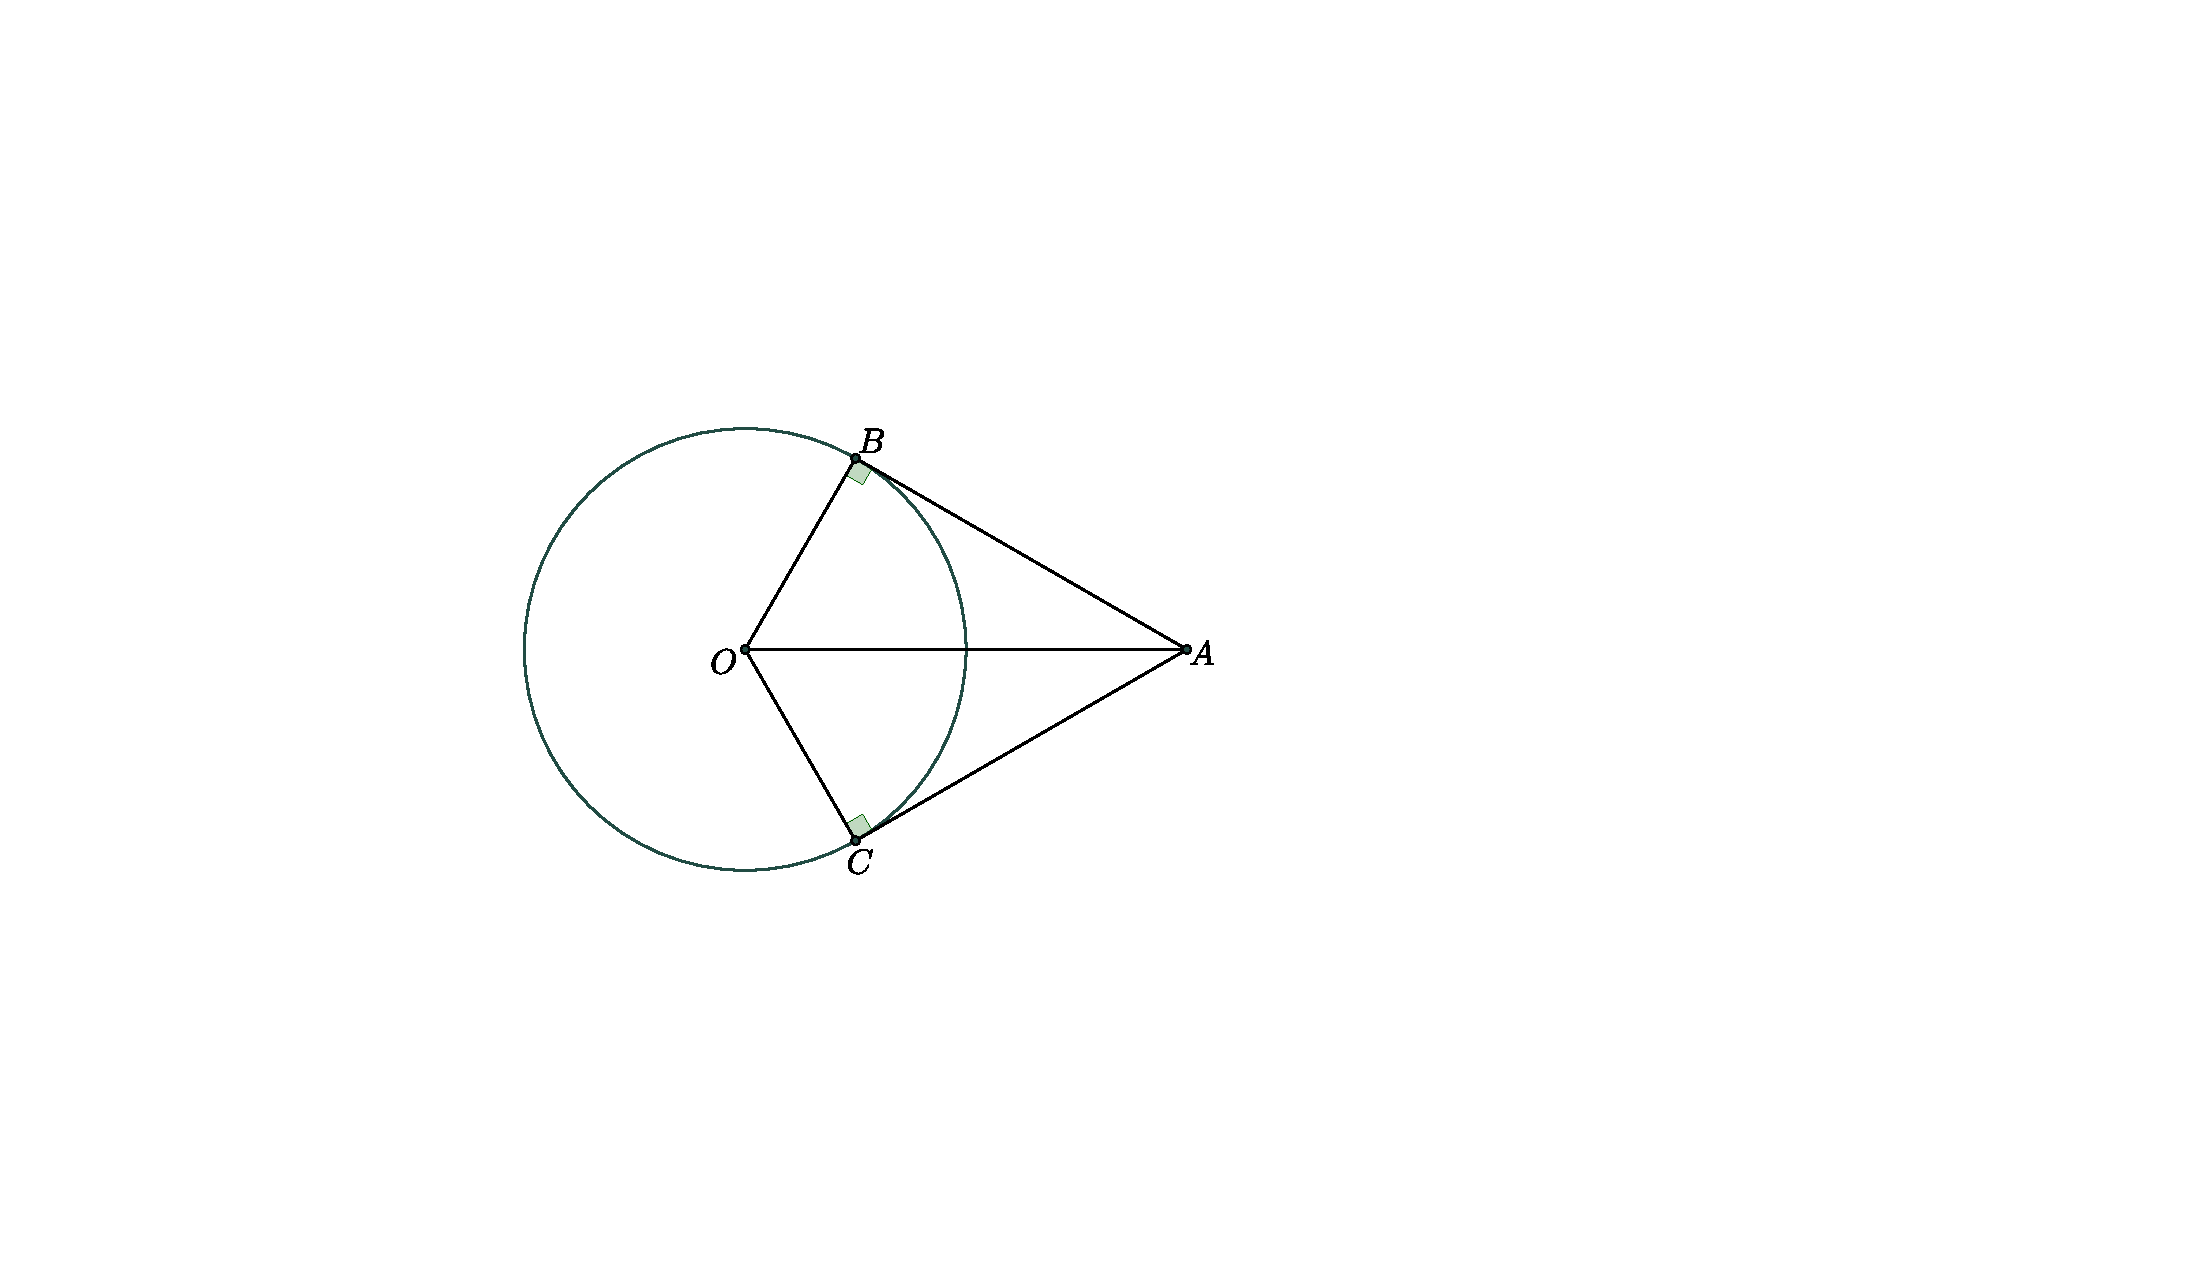
\includegraphics[width=0.9\marginparwidth]{img/tinh_chat_hai_tiep_tuyen_cat_nhau.pdf}
	\vspace{0.5cm}
	\margincaption{Tính chất hai tiếp tuyến cắt nhau}
	\label{hinh2.5}
\end{marginfigure}
\hq{
Ta có thể hiểu tính chất này một cách đơn giản như sau. Nếu 2 tiếp tuyến $AB$ và $AC$ cắt nhau tại $A$ \xd $\suyra$ 
$\begin{cases}
	AB = AC \xd
	\goc{BAO} = \goc{CAO} \xd
	\goc{BOA} = \goc{COA}
\end{cases}$ 
}{
\begin{center}
	Xét $\tamgiac AOB$ và $\tamgiac AOC $, có:\xd
$\begin{cases}
	AO \text{ là cạnh chung}\xd
	OB=OC~(=R)
\end{cases}$
\xd
$\suyra \tamgiac AOB = \tamgiac AOC~(ch-cgv)$\xd
$\suyra \begin{cases}
	AB = AC\xd
	\goc{BAO} = \goc{CAO}\xd
	\goc{BOA} = \goc{COA}
\end{cases}$
\end{center}
}

\begin{smallfont}
	\ex{Bài toán kinh điển}{
	Cho $(O; R)$ và 2 tiếp tuyến $AB; AC$ ($A$ nằm ngoài $(O; R)$)
	\begin{enumerate}[label=\alph*)]
		\item Chứng minh: $OA \vuong BC$.
		
		\item Gọi $H$ là giao điểm của $OA$ và $BC$. Chứng minh: $OB^2 = OH.OA$.
		
		\item Gọi $D \thuoc (O; R)$ ($D \khac B; C $). Chứng minh: $OD^2 = OH.OA$. 
	\end{enumerate}
	}
	
	\textbf{\textit{Lời giải:}}
		\begin{enumerate}[label=\alph*)]
			\item $\begin{cases}
				OB = OC = R \xd
				AB = AC ~(\textit{Tính chất 2 tiếp tuyến cắt nhau})
			\end{cases}$ \xd
			$\suyra$ $OA$ là đường trung trực của $BC$ \xd
			$\suyra$ \colorbox{themecolor!10!white}{$OA \vuong BC$}
			\item Xét $\tamgiac ABO$ và $\tamgiac BHO$, có: \xd
			$\begin{cases}
				\goc O \text{~chung} \xd
				\goc{ABO} = \goc{BHO} = 90^\circ
			\end{cases}$ \xd
			$\suyra \tamgiac ABO \dongdang \tamgiac BHO~(g-g)$ \xd
			$\suyra \frac{AB}{BH} = \frac{BO}{HO} = \frac{AO}{BO} \suyra \frac{BO}{HO} = \frac{AO}{BO}$ \xd
			$\suyra$ \colorbox{themecolor!10!white}{$OB^2 = OH.OA$}
			\item Có: $OD = OB = R$ \xd
			mà $OB^2 = OH.OA$ \xd
			$\suyra$ \colorbox{themecolor!10!white}{$OD^2 = OH.OA$} \qed
		\end{enumerate}
   
 	\begin{marginfigure}|-12cm|
		\centering
		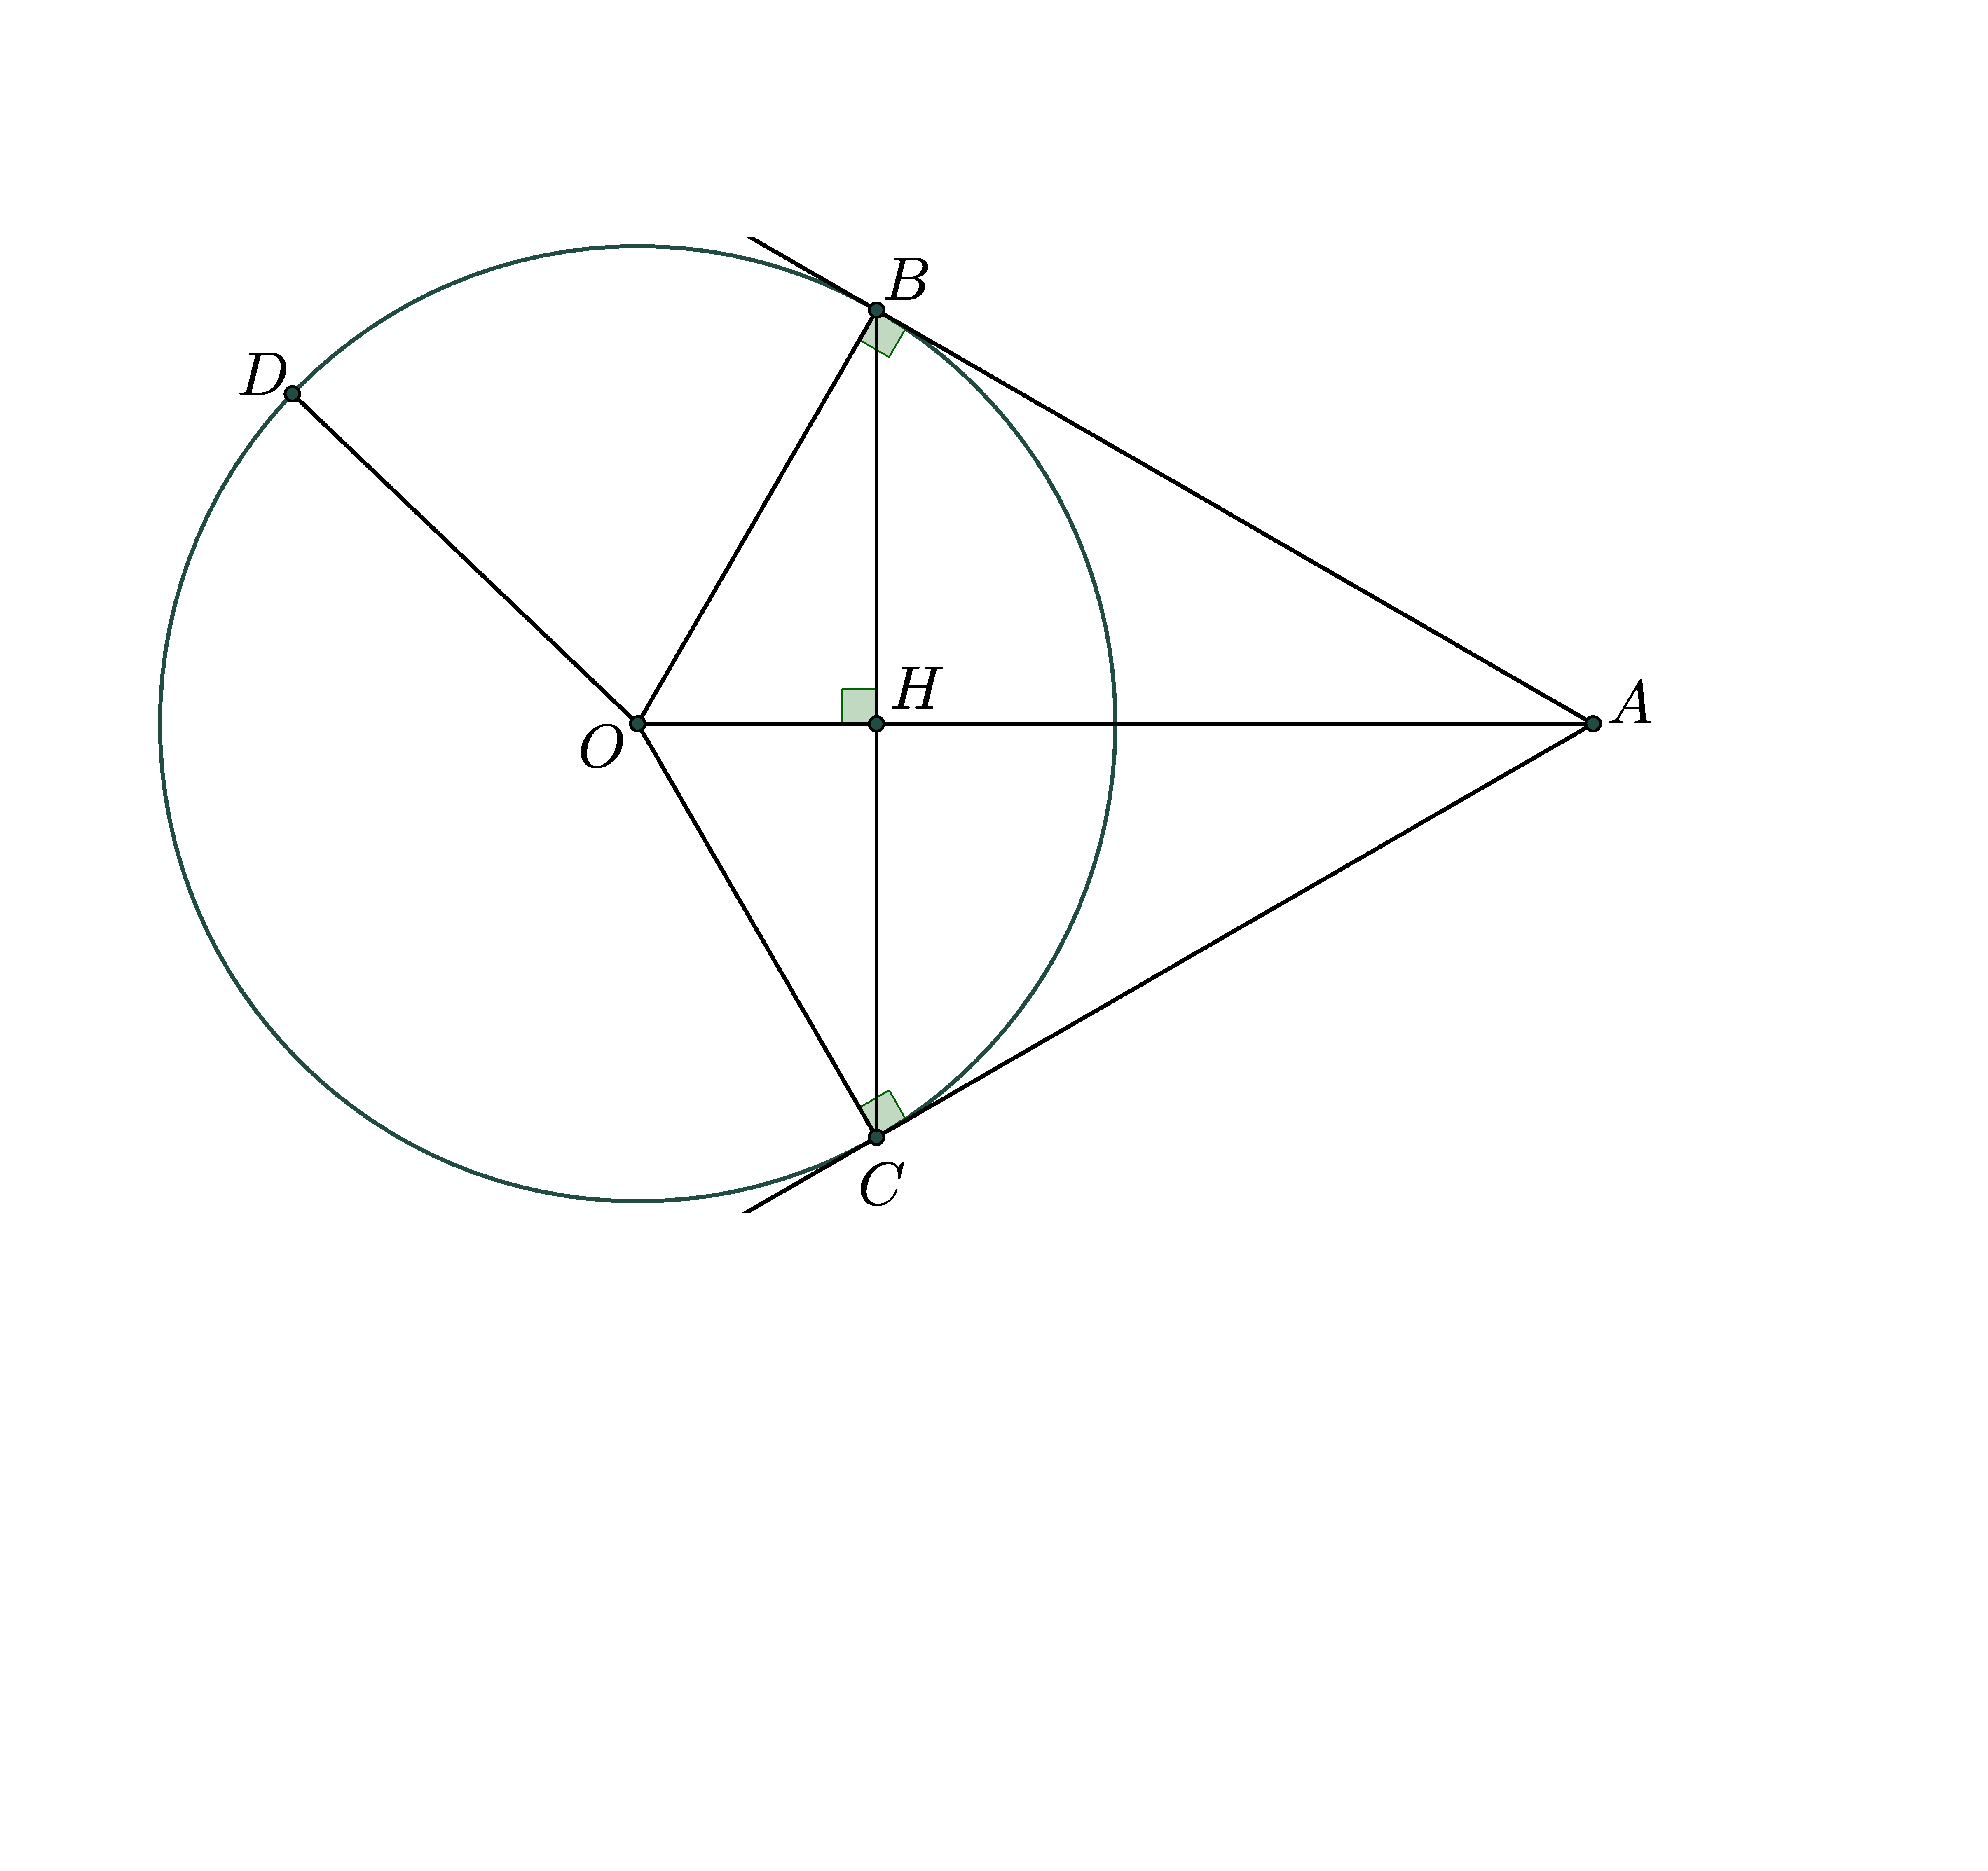
\includegraphics[width=0.8\marginparwidth]{img/vi_du_1.pdf}
		\vspace{0.5cm}
		\margincaption{Ví dụ 1}
		\label{hinh2.6c}
	\end{marginfigure}
\end{smallfont}

\baitap
\begin{smallfont}
%-----Bài 1-----%
    \bt[CTST Tr.88]{
    $AB$ là tiếp tuyến của $(O)$ tại $B$ 
	\begin{enumerate}[label=\alph*)]
		\item 
		Tính bán kính $r$ của $(O)$.
		\item 
		Tính chiều dài cạnh $OA$ của tam giác $ABO$.
	\end{enumerate}
    \textbf{\textit{Gợi ý:}}
    \begin{enumerate}[label=\alph*)]
		\item 
		Có tiếp tuyến nên sẽ có vuông góc, mà đề lại yêu cầu tính cạnh, vậy ta sẽ dùng định lý Pythagoras.
		\item 
		Khi tìm được đáp án của câu a ta sử dụng cộng cạnh với cạnh để tìm $OA$.
	\end{enumerate}
    }
%-----Hình bài 1-----%
\begin{marginfigure}|-4.5cm|
		\centering
		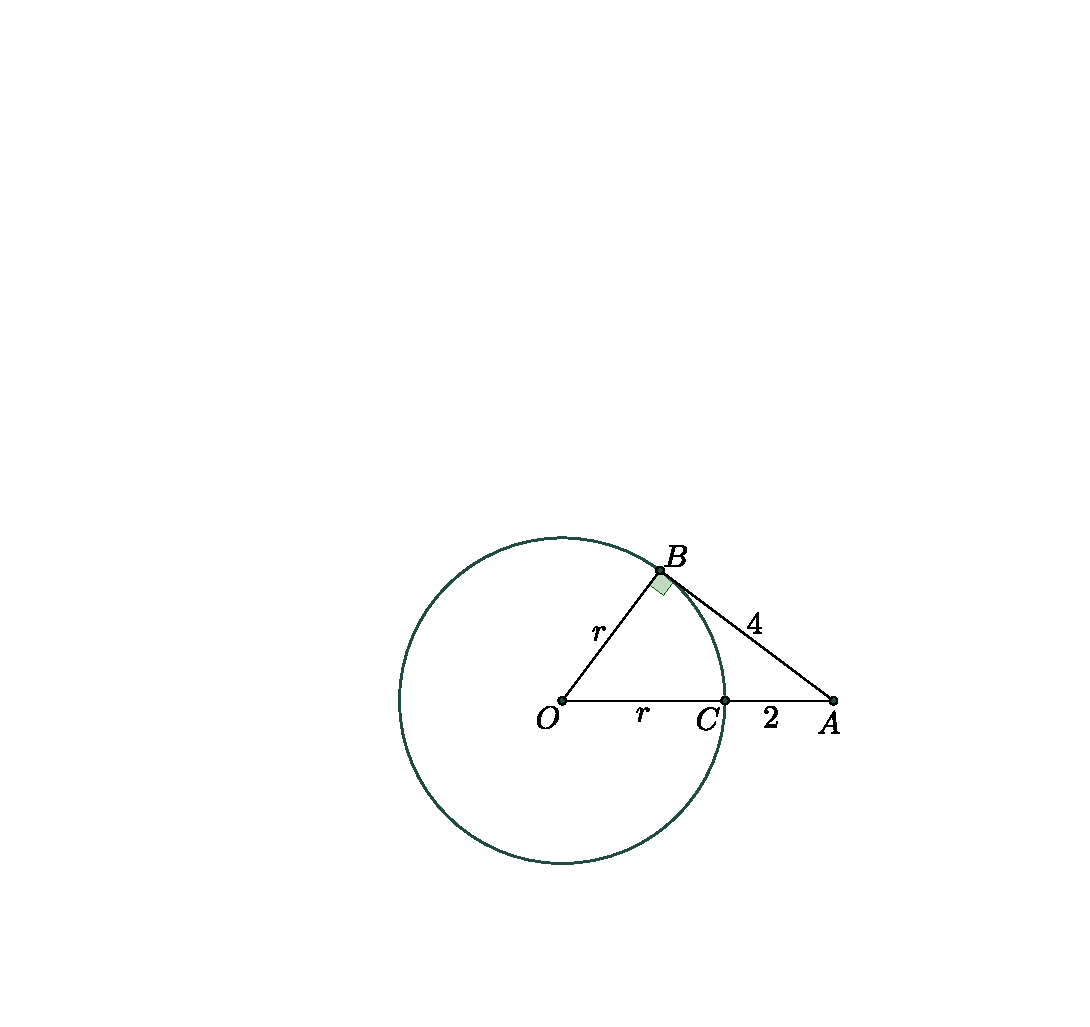
\includegraphics[width=0.7\marginparwidth]{imgc2/Bai1.pdf}
		\vspace{0.2cm}
		\margincaption{Bài 1}
		\label{hinh2.7}
\end{marginfigure}
\xdd

%-----Bài 2-----%
\bt[CTST Tr.88]{
    $MB$, $MC$ lần lượt là tiếp tuyến của đường tròn $(O)$ tại $B, C$; $\goc{COB} = 130^\circ $. Tính số đo $\goc{CMB}$. \xd
    \textbf{\textit{Gợi ý:}} \xd
    Có tiếp tuyến nên có vuông góc từ đó biết được số đo của 2 góc $B, C$ là $90^\circ$. Mà $\goc{CMB}$ nằm trong tứ giác $OBMC$. Vậy ta sẽ sử dụng tổng 4 góc trong tứ giác.
}
%-----Hình bài 2-----%
\begin{marginfigure}|-3.5cm|
		\centering
		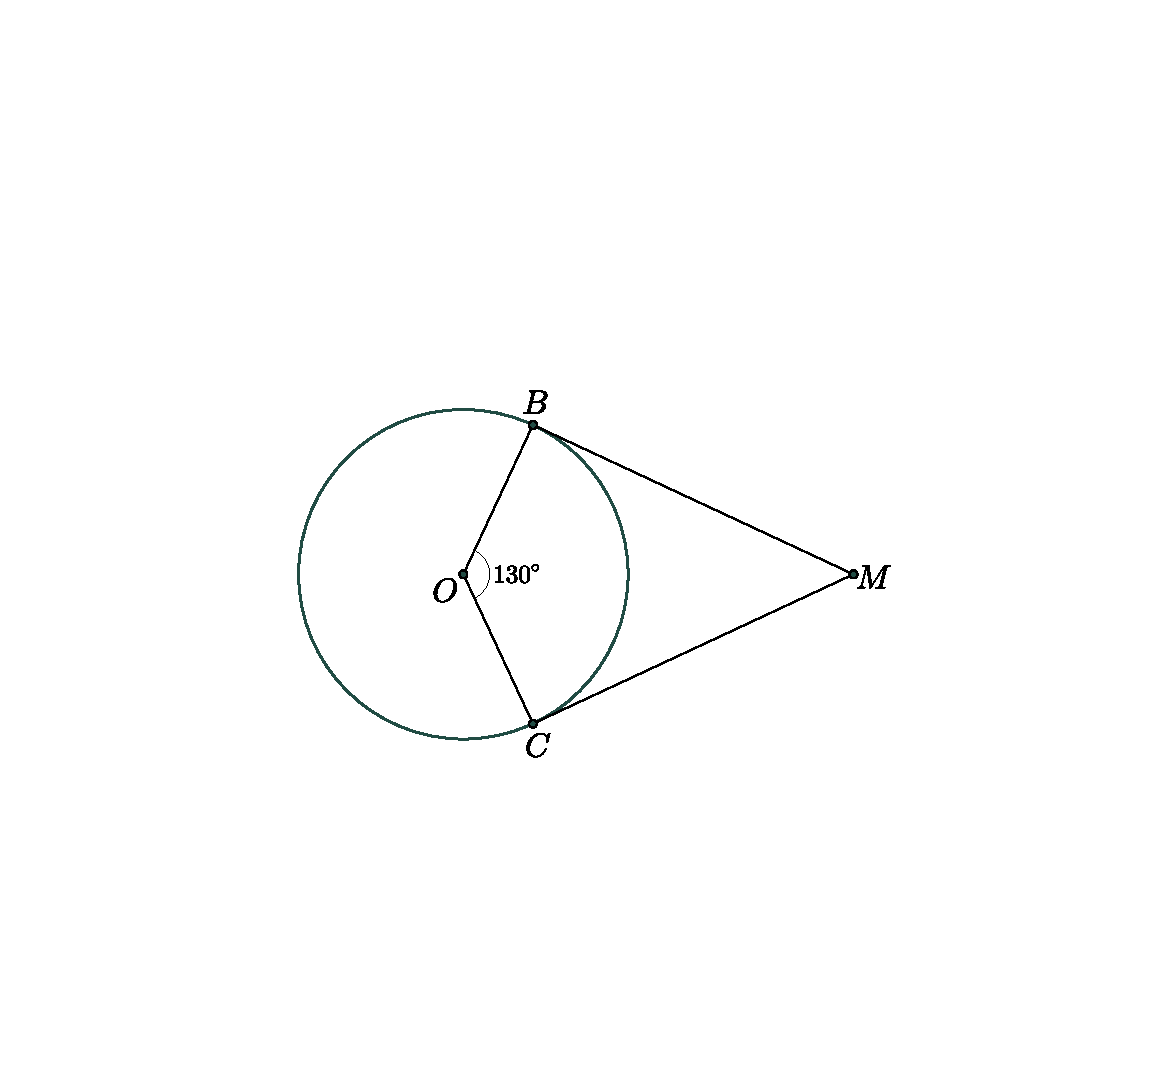
\includegraphics[width=0.8\marginparwidth]{imgc2/Bai2.pdf}
		\vspace{0.2cm}
		\margincaption{Bài 2}
		\label{hinh2.8}
\end{marginfigure}
\xdd
%-----Bài 3-----%
\bt[CTST Tr.88]{
    Biết $AB$, $AC$ lần lượt là tiếp tuyến của đường tròn $(O)$ tại $B, C$. Tính giá trị của $x$. \xd
    \textbf{\textit{Gợi ý:}} \xd
    Nhận thấy 2 tiếp tuyến $AB, AC$ cắt nhau tại $A$ nên ta sử dụng tính chất 2 tiếp tuyến cắt nhau.
    }
%-----Hình Bài 3-----%
\begin{marginfigure}|-3cm|
		\centering
		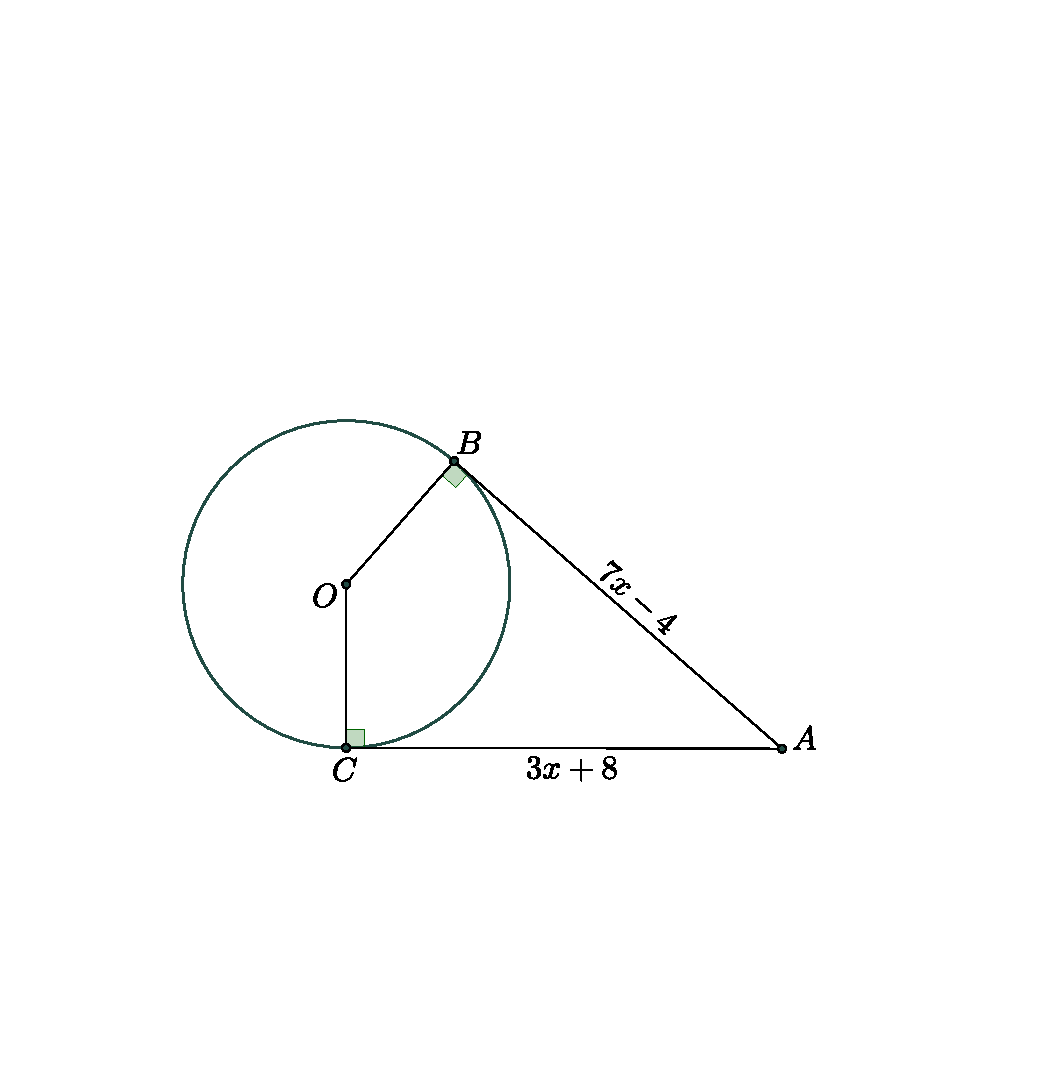
\includegraphics[width=0.8\marginparwidth]{imgc2/Bai3.pdf}
		\vspace{0.2cm}
		\margincaption{Bài 3}
		\label{hinh2.9}
\end{marginfigure}
\xdd

%-----Bài 4-----%
\bt[CTST Tr.89]{
    $AB = 9, BC = 12, AC = 15$ và $BC$ là đường kính của đường tròn $(O)$. Chứng minh $AB$ là tiếp tuyến của đường tròn $(O)$. \xd
	\textbf{\textit{Gợi ý:}} \xd
    \textbullet Khi đề bài cho 3 cạnh của một tam giác thì đó không phải sự ngẫu nhiên mà đề bài muốn ta sử dụng định lí Pythagoras đảo nhằm kiểm tra đó có phải tam giác vuông hay không. \xd
	\textbullet Để chứng minh tiếp tuyến ta chỉ có một hướng đi là chứng minh đường thẳng đó vuông góc với bán kính tại một điểm thuộc đường tròn.
	}
%-----Hình Bài 4-----%
\begin{marginfigure}|-4cm|
		\centering
		\includegraphics[width=0.7\marginparwidth]{imgc2/Bai4.pdf}
		\vspace{0.2cm}
		\margincaption{Bài 4}
		\label{hinh2.10}
\end{marginfigure}	
\xdd

\bt[CTST Tr.89]{
    Cho tam giác $ABC$ có đường tròn $(O)$ nằm trong và tiếp xúc với ba cạnh của tam giác. Biết $AM = 6~cm, BP = 3~cm, CE = 8~cm$. Tính chu vi tam giác $ABC$. \xd
    \textbf{\textit{Gợi ý:}} \xd
	\textbullet Để tính chu vi ta cần nhớ rằng "Chu vi bằng tất cả các cạnh cộng lại". Vậy để tính được chu vi $\tamgiac ABC$ ta cần tính được 3 cạnh là $AB, AC, BC$. \xd
	\textbullet Nhận thấy rằng ta có 3 tiếp tuyến với các tiếp điểm là $M, E, P$. Sử dụng tính chất 2 tiếp tuyến cắt nhau cho các cặp tiếp tuyến $(AM, AE); (BM, BP); (CE; CP)$. \xd
	\textbullet Dùng cộng cạnh hoặc trừ cạnh để tìm 3 cạnh $AB, AC, BC$.
	}
%-----Hình Bài 5-----%
\begin{marginfigure}|-4cm|
		\centering
		\includegraphics[width=0.8\marginparwidth]{imgc2/Bai5.pdf}
		\vspace{0.2cm}
		\margincaption{Bài 5}
		\label{hinh2.11}
\end{marginfigure}	
\xdd

\bt[CTST Tr.89]{
    Cho đường tròn $(O; R)$ có đường kính $AB$. Vẽ dây $AC$ sao cho $AC = R$. Gọi $I$ là trung điểm của dây $AC$. Đường thẳng $OI$ cắt tiếp tuyến $Ax$ tại $M$. Chứng minh rằng:
	\begin{enumerate}[label=\alph*)]
		\item  
		$\goc{ACB}$ có số đo bằng $90^\circ$, từ đó suy ra độ dài của $BC$ theo $R$;
		    
		\item
		$OM$ là tia phân giác của $\goc{COA}$;
		
		\item
		$MC$ là tiếp tuyến của đường tròn $(O; R)$.
	\end{enumerate}
}
\xdd

\bt[CTST Tr.89]{
    Cho đường tròn $(O; 5~cm)$, điểm $M$ nằm ngoài $(O)$ sao cho hai tiếp tuyến $MA$ và $MB$ ($A, B$ là hai tiếp điểm) vuông góc với nhau tại M
	\begin{enumerate}[label=\alph*)]
		\item  
		Tính độ dài của $MA$ và $MB$.
		
		\item
		Qua giao điểm $I$ của đoạn thẳng $MO$ và đường tròn $(O)$, vẽ một tiếp tuyến cắt $OA, OB$ lần lượt tại $C, D$. Tính độ dài của $CD$.
	\end{enumerate}
}
\xdd

\bt[CTST Tr.89]{
    Cho đường tròn $(O)$, điểm $M$ nằm ngoài $(O)$ sao cho $MA$ và $MB$ là hai tiếp tuyến ($A, B$ là hai tiếp điểm) thoả mãn $\goc{AMB} = 60^\circ$. Biết chu vi tam giác $MAB$ là $18~cm$, tính độ dài dây $AB$.
}
\end{smallfont}

\subsection{Dạng 1: Chứng minh một đường thẳng là tiếp tuyến}
\begin{smallfont}
	\bt[TOANMATH]{Cho tam giác $ABC$ có $AB = 6cm, AC = 8cm, BC = 10cm$. Vẽ đường tròn $(B; BA)$. Chứng minh $AC$ là tiếp tuyến của đường tròn $(B)$.}
	\xdd
	
	\bt[Tiến Sĩ Trần Hoan]{Cho $\tamgiac$ $ABC$ có $AB= 3cm; AC = 4cm; BC = 5cm$. Chứng minh rằng $AC$ là tiếp tuyến của đường tròn $(O)$.}
	\xdd
	
	\bt[Tiến Sĩ Trần Hoan]{Từ điểm $A$ nằm ngoài $(O;R)$ vẽ tiếp tuyến $AB$ ($B$ là tiếp điểm); lấy $C$ trên đường tròn sao cho $AB = AC$. Chứng minh rằng $AC$ là tiếp tuyến của đường tròn.
	}
	\xdd
	
	\bt[Tiến Sĩ Trần Hoan]{Cho (O); vẽ dây $BC$ khác đường kính; qua $O$; kẻ đường thẳng vuông góc với $BC$ cắt tiếp tuyến tại $B$ của đường tròn ở $A$. Chứng minh rằng $AC$ là tiếp tuyến của $(O)$.}
	\xdd 

	\bt[Tiến Sĩ Trần Hoan]{Cho $(O)$; đường kính $AB$. Kẻ tiếp tuyến tại $B$ với $(O)$; trên tiếp tuyến lấy $P$. Qua $A$ kẻ đường thẳng song song với $OP$; cắt $(O)$ tại $Q$. Chứng minh $PQ$ là tiếp tuyến $(O)$.}
	\xdd 

	\bt[Thạc Sĩ Nguyễn Văn Hòa]{Từ một điểm $A$ nằm ngoài đường tròn $(O; R)$; vẽ tiếp tuyến $AB$($B$ là tiếp điểm). Kẻ dây $BC$ vuông góc với $OA$. Chứng minh $AC$ là tiếp tuyến của đường tròn.}
	\xdd
	
	\bt[Thạc Sĩ Nguyễn Văn Hòa]{Cho đường tròn tâm $O$ và đường kính $AB$. Một điểm $M$ nằm trên đường thẳng $AB$ ($A$ nằm giữa $M$ và $B$), qua điểm $M$ kẻ đường thẳng $MC$ tiếp xúc với đường tròn $(O)$ tại $C$. Từ $O$ dựng đường vuông góc với $BC$ cắt $MC$ tại $N$. Chứng minh đường thẳng $NB$ là tiếp tuyến của $(O)$.}
	\xdd 

	\bt[Thạc Sĩ Nguyễn Văn Hòa]{Cho 3 điểm $A; B; C$ cùng thuộc (O) sao cho $\tamgiac ABC$ cân tại $A$. Vẽ hình bình hành $ABCD$. Chứng minh $AD$ là tiếp tuyến của $(O)$.}
	\xdd 

	\bt[Internet]{Cho tam giác $ABC$ cân tại $A$ đường cao $BH$. Trên mặt phẳng chứa $C$ bờ $AB$ vẽ $Bx \vuong BA$ cắt đường tròn tâm $B$ bán kính $BH$ tại $D$. Chứng minh $CD$ là tiếp tuyến của $(B)$.}
	\xdd

	\bt[Internet]{Cho hình thang vuông $ABCD; (\goc{A}=\goc{B}=90^\circ)$ có $O$ là trung điểm của $AB$ và góc $\goc{COD} = 90^\circ$. Chứng minh $CD$ là tiếp tuyến của đường tròn đường kính $AB$.}
\end{smallfont}


%----- CHƯƠNG 3 -----%
\setchapterabstract{Bài học giới thiệu về các bài toán về việc giải quyết một số vấn đề gần gũi với đời sống bằng kiến thức toán học cơ bản. Các chủ đề tiêu biểu là: chuyển động, diện tích, năng suất, tiền tệ, hình khối,...}
\chapter{TOÁN THỰC TẾ}
\chaptoc[0.68cm]
\section{Toán chuyển động}
Cái bài toán liên quan đến toán chuyển động tập trung xoay quanh vào mối quan hệ giữa 3 đại lượng là $v-$vận tốc, $s-$quãng đường, $t-$thời gian. Vì vậy trong chủ đề này ta chỉ tập trung xoay quanh một công thức duy nhất:
\[
    \colorbox{themecolor!10!white}{$v = \frac{s}{t}$}
\]

\begin{smallfont}
    \bt[TUYỂN SINH SÓC TRĂNG 2022-2023]
    {
        \textit{Năm 2021 Thủ tướng chính phủ đã phê duyệt dự án xây dựng công trình đường cao tốc Châu Đốc - Cần Thơ - Sóc Trăng, dự án này có ý nghĩa đặc biệt quan trọng, sẽ góp phần phát triển kinh tế xã hội của tỉnh Sóc Trăng nói riêng và khu vực đồng bằng Sông Cửu Long nói chung.} Theo ước tính chiều dài toàn tuyến cao tốc từ Châu Đốc đến Sóc Trăng là $188~km$. Biết rằng vận tốc ô tô đi trên đường cao tốc lớn hơn vận tốc ô tô đi trên quốc lộ là $34~km/h$. Vì vậy nếu ô tô di chuyển trên quãng đường $188~km$ thì việc di chuyển trên đường cao tốc sẽ rút ngắn được 68 phút so với việc di chuyển trên quốc lộ. Tính vận tốc của ô tô khi di chuyển trên đường cao tốc.
    }
    \xdd
    \bt[TUYỂN SINH SÓC TRĂNG 2025-2026]
    {
        Vào lúc 6 giờ sáng, ông An đi ô tô xuất phát từ nhà tại Vị Thanh để đến cơ quan làm việc ở Cần Thơ cách nhà $50~km$. Cùng lúc đó ông Bình đi ô tô từ nhà tại Sóc Trăng đến cùng cơ quan làm việc với ông An cách nhà $60~km.$ Biết rằng ông Bình đi với tốc độ lớn hơn tốc độ của ông An là $10~km/h$ nên đã đến cơ quan cùng lúc với ông An. Hỏi ông An và ông Bình đến cơ quan lúc mấy giờ?
    }
    \xdd
    \bt[TUYỂN SINH BÀ RỊA VŨNG TÀU 2018-2019]
    {
        Hai ô tô khởi hành cùng một lúc từ thành phố $A$ đến thành phố $B$ cách nhau $450~km$ với vận tốc không đổi. Vận tốc xe thứ nhất lớn hơn vận tốc xe thứ hai $10~km/h$ nên xe thứ nhất đến trước xe thứ hai 1,5 giờ. Tính vận tốc mỗi xe.
    }
    \xdd 
    \bt[TUYỂN SINH BÀ RỊA VŨNG TÀU 2022-2023]
    {
        Một người đi xe máy từ điểm $A$ đến địa điểm $B$ trên quãng đường $100~km$. Khi từ $B$ về $A$ người đó đã giảm vận tốc $10~km/h$ so với lúc đi nên thời gian lúc về nhiều hơn thời gian lúc đi là 30 phút. Tính vận tốc của người đó lúc đi.
    }
    \xdd 
    \bt[TUYỂN SINH ĐỒNG THÁP 2018-2019]
    {
        Để chuẩn bị cho mùa giải sắp tới, một vận động viên đua xe ở Đồng Tháp đã luyện tập leo dốc và đổ dốc trên cầu Cao Lãnh. Biết rằng đoạn leo đốc và đổ dốc ở hai bên đầu cầu có độ dài cùng bằng $1~km$. Trong một lần luyện tập, vận động viên khi đổ dốc nhanh hơn vận tốc khi leo dốc là $9~km/h$ và tổng thời gian hoàn thành là 3 phút. Tính vận tốc leo dốc của vận động viên trong lần tập luyện đó.
    }
    \xdd 
    \bt[TUYỂN SINH ĐỒNG THÁP 2025-2026]
    {
        Một người lái xe đi từ $A$ đến $B$ cách nhau $90~km$ với tốc độ và thời gian dự định. Nhưng vì trời mưa, xe đi với tốc độ chậm hơn dự định $15~km/h$ nên thời gian đi đến $B$ nhiều hơn dự định 30 phút. Tính tốc độ dự định và tốc độ thực tế xe đi từ $A$ đến $B$.
    }
    \xdd 
    \bt[TUYỂN SINH ĐỒNG NAI 2021-2022]
    {
        Hằng ngày bạn Mai đi học bằng xe đạp, quãng đường từ nhà đến trường dài $3~km$. Hôm nay, xe đạp hư nên Mai nhờ mẹ chở đi đến trường bằng xe máy với vận tốc lớn hơn vận tốc khi đi xe đạp là $24~km/h$, cùng một thời điểm khởi hành như mọi ngày nhưng Mai đã đến trường sớm hơn 10 phút. Tính vận tốc của bạn Mai khi đi học bằng xe đạp.
    }
    \xdd 
    \bt[TUYỂN SINH KIÊN GIANG 2021-2022]
    {
        Một ô tô chở khách dự định đi từ thành phố Rạch Giá đến thành phố Hà Tiên trên quãng đường dài $90~km$ trong một thời gian đã định. Sau khi đi 1 giờ, ô tô ghé trạm dừng chân nghỉ 10 phút, do đó để đến thành phố Hà Tiên như dự định, người lái xe ô tô tăng vận tốc thêm $9~km/h$. Tính vận tốc lúc đầu của ô tô.
    }
    \xdd 
    \bt[TUYỂN SINH TIỀN GIANG 2019-2020]
    {
        Hai người đi xe đạp từ huyện $A$ đến huyện $B$ trên quãng đường dài $24~km$, khởi hành cùng một lúc. Vận tốc xe của người thứ nhất hơn vận tốc xe của người thứ hai là $3~km/h$ nên người thứ nhất đến huyện $B$ trước người thứ hai là 24 phút. Tính vận tốc của mỗi người.
    }
    \xdd 
    \bt[TUYỂN SINH TIỀN GIANG 2022-2023]
    {
        Một xe tải đi theo hướng từ $A$ đến $B$ cách nhau $210~km$. Sau 2 giờ, cũng trên quãng đường đó, một ô tô khởi hành theo hướng từ $B$ đến $A$ với vận tốc lớn hơn vận tốc xe tải $10~km/h$. Tính vận tốc của xe tải, biết hai xe gặp nhau tại nơi cách $A$ một khoảng bằng $150~km$.
    }
    \xdd 
    \bt[TUYỂN SINH TIỀN GIANG 2020-2021]
    {
        Một người đi xe máy từ địa điểm $A$ đến địa điểm $B$ hết 1 giờ 30 phút, rồi tiếp tục đi từ địa điểm $B$ đến địa điểm $C$ hết 2 giờ. Tìm vận tốc của người đi xe máy trên mỗi quãng đường $AB$ và $BC$, biết quãng đường xe máy đã đi từ $A$ đến $C$ dài $150~km$ và vận tốc của xe máy đi trên quãng đường $AB$ nhỏ hơn vận tốc đi trên quãng đường $BC$ là $5~km/h$
    }
    \xdd 
    \bt[TUYỂN SINH BÌNH DƯƠNG 2018-2019]
    {
        Một người dự định đi xe máy từ tỉnh $A$ đến tỉnh $B$ cách nhau $90~km$ trong một thời gian đã định. Sau khi đi được 1 giờ người đó nghỉ 9 phút. Do đó, để đến tỉnh $B$ đúng hẹn, người ấy phải tăng vận tốc thêm $4~km/h$. Tính vận tốc lúc đầu của người đó.
    }
    \xdd 
    \bt[TUYỂN SINH NGHỆ AN 2019-2020]
    {
        Tình cảm gia đình có sức mạnh thật phi thường. Bạn Vi Quyết Chiến - Cậu bé 13 tuổi quá thương nhớ em trai của mình đã vượt qua một quãng đường dài $180~km$ từ Sơn La đến bệnh viện nhi Trung ương Hà Nội để thăm em. Sau khi đi bằng xe đạp 7 giờ, bạn ấy được lên xe khách và đi tiếp 1 giờ 30 phút nữa thì đến nơi. Biết vận tốc của xe khách lớn hơn vận tốc của xe đạp là $35~km/h$. Tính vận tốc xe đạp của bạn Chiến.      
    }
    \xdd 
    \bt[TUYỂN SINH PHÚ YÊN 2019-2020]
    {
        Một người đi xe máy từ thị trấn Chí Thạnh đến thị trấn Hai Riêng với vận tốc dự định trước. Sau khi đi được $\frac{1}{3}$ quãng đường, vì đoạn đường còn lại xấu nên người đó phải đi với vận tốc nhỏ hơn so với dự định $10~km/h$, do đó đến thị trấn Hai Riêng muộn hơn dự định 18 phút. Tính vận tốc dự định, biết rằng quãng đường từ thị trấn Chí Thạnh đến thị trấn Hai Riêng là $90~km$.
    }
    \xdd 
    \bt[TUYỂN SINH PHÚ YÊN 2022-2023]
    {
        Phú và Yên cùng tham gia cuộc thi ma-ra-tông cự li $10~km$. Trong $4~km$ đầu, cả hai chạy cùng một vận tốc. Trong $6~km$ cuối, Phú tăng vận tốc thêm $2~km/h$. Yên vẫn duy trì vận tốc của mình trong suốt quãng đường đua. Kết quả là Phú về đích sớm hơn Yên 6 phút. Tính vận tốc chạy của Yên.
    }
    \xdd 
    \bt[TUYỂN SINH THỪA THIÊN HUẾ 2024-2025]
    {
        Hai học sinh cùng tham gia một giải chạy với hai cự li khác nhau, cự li của học sinh thứ nhất gấp đôi cự li của học sinh thứ hai (cự li là quãng đường mà người chạy phải hoàn thành). Biết rằng học sinh thứ nhất mất trung bình 5 phút để chạy hết $1~km$, học sinh thứ hai mất trung bình 7 phút đễ chạy hết $1~km$ và thời gian hoàn thành cự li của học sinh thứ nhất nhiều hơn thời gian hoàn thành cự li của học sinh thứ hai là 15 phút. Tính cự li của mỗi học sinh tham gia.
    }
    \xdd 
    \bt[TUYỂN SINH LAI CHÂU 2025-2026]
    {
        Một người đi xe máy từ Than Uyên đến Tam Đường. Khi đi được quãng đường $40~km$ đến Tân Uyên người đó dừng lại nghỉ 20 phút rồi đi tiếp $30~km$ nữa để đến Tam Đường với vận tốc lớn hơn vận tốc khi đi từ Than Uyên đến Tân Uyên là $5~km/h$. Tính vận tốc của người đi xe máy khi đi từ Than Uyên đến Tân Uyên, biết tổng thời gian đi từ Than Uyên đến Tam Đường là 2 giờ.
    }
    \xdd 
    \bt[TUYỂN SINH CAO BẰNG 2024-2025]
    {
        Bạn Hưng đi xe đạp từ nhà đến trường với quãng đường $10~km$. Khi đi từ trường về nhà, vẫn trên cung đường ấy, do lượng xe tham gia giao thông nhiều hơn nên bạn Hưng phải giảm vận tốc $2~km/h$ so với khi đến trường. Vì vậy thời gian về nhà nhiều hơn thời gian đến trường là 10 phút. Tính vận tốc của xe đạp khi bạn Hưng đi từ nhà đến trường và từ trường về nhà.
    }
    \xdd 
    \bt[TUYỂN SINH VĨNH PHÚC 2019-2020]
    {
        Người thứ nhất đi đoạn đường từ địa điểm $A$ đến địa điểm $B$ cách nhau $78~km$. Sau khi người thứ nhất đi được 1 giờ thì người thứ hai đi theo chiều ngược lại vẫn trên đoạn đường đó từ $B$ về $A$. Hai người gặp nhau ở địa điểm $C$ cách $B$ một quãng đường $36~km$. Tính vận tốc của mỗi người, biết rằng vận tốc của người thứ hai lớn hơn vận tốc của người thứ nhất là $4~km/h$ và vận tốc của mỗi người trong suốt đoạn đường là không thay đổi.
    }
    \xdd 
    \bt[TUYỂN SINH LÀO CAI 2022-2023]
    {
        Hai ô tô xuất phát cùng một thời điểm từ địa điểm $A$ đến địa điểm $B$ với vận tốc mỗi ô tô không đổi. Sau 1 giờ quãng đường đi được của ô tô thứ nhất nhiều hơn quãng đường đi được của ôtô thứ hai là $5~km$. Quãng đường đi được của ô tô thứ hai sau 3 giờ nhiều hơn quãng đường đi được của ô tô thứ nhất sau 2 giờ là $35~km$. Tính vận tốc mỗi ô tô.
    }
    \xdd 
    \bt[TUYỂN SINH HỒ CHÍ MINH 2025-2026]
    {
        Từ vị trí $A$ của một công viên có dạng hình vuông $ABCD$ cạnh $a~km$, hai bạn Hòa và Bình bắt đầu chạy bộ cùng lúc với vận tốc không đổi dọc theo các cạnh của hình vuông và theo hai hướng khác nhau. Biết rằng, hai bạn gặp nhau lần thứ nhất tại vị trí $E$ cách $A$ một khoảng bằng $1~km$ và gặp lại nhau lần thứ hai tại vị trí $F$ cách $A$ một khoảng bằng $0,4~km$ như hình vẽ. Gọi $x, y~(km/h)$ lần lượt là vận tốc của Hòa và Bình.
        \begin{enumerate}[label=\alph*)]
		    \item 
		    Chứng minh rằng $\frac{x}{y} = \frac{AB + BC + CE}{AD + DE}$.
		    \item 
		    Tìm giá trị của $a$.
	    \end{enumerate}
    }
    \xdd 
        \begin{marginfigure}|-4.5cm|
		    \centering
		    \includegraphics[width=0.7\marginparwidth]{imgc2/HCM25256.pdf}
		    \vspace{0.2cm}
		    \margincaption{Bài 21}
        \end{marginfigure}
    \bt[TUYỂN SINH BÀ RỊA VŨNG TÀU 2019-2020]
    {
        Có một vụ tai nạn ở vị trí $B$ tại chân của một ngọn núi (chân núi có dạng đường tròn tâm $O$, bán kính $3~km$) và một trạm cứu hộ ở vị trí $A$ (tham khảo hình vẽ). Do chưa biết đường nào để đến vị trí tai nạn nhanh hơn nên đội cứu hộ quyết định điều hai xe cứu thương cùng xuất phát ở trạm đến vị trí tai nạn theo hai cách sau \xd  
        Xe thứ nhất: đi theo đường thẳng từ $A$ đến $B$, do đường xấu nên vận tốc trung bình của xe là $40~km/h$. \xd 
        Xe thứ hai: đi theo đường thẳng từ $A$ đến $C$ với vận tốc trung bình $60~km/h$, rồi đi từ $C$ đến $B$ theo đường cung nhỏ $CB$ ở chân núi với vận tốc trung bình $30~km/h$ (3 điểm $A, O, C$ thẳng hàng và $C$ ở chân núi). Biết đoạn đường $AC$ dài $27~km$ và  $\goc{ABO} = 90^\circ$.
        \begin{enumerate}[label=\alph*)]
		    \item 
		    Tính độ dài quãng đường xe thứ nhất đi từ $A$ đến $B$.
		    \item 
		    Nếu 2 xe cứu thương xuất phát cùng một thời điểm tại $A$ thì xe nào đến vị trí tai nạn trước?
	    \end{enumerate}
    }
    \xdd 
        \begin{marginfigure}|-5.6cm|
		    \centering
		    \includegraphics[width=\marginparwidth]{imgc2/BRVT1920.pdf}
		    \vspace{0.2cm}
		    \margincaption{Bài 22}
        \end{marginfigure}
    \bt[THAM KHẢO]
    {
    Trong một công viên hình tam giác đều $ABC$ cạnh $4~km$, hai vận động viên Lan và Minh xuất phát cùng lúc từ đỉnh $A$. Lan chạy theo chiều kim đồng hồ với vận tốc $6~km/h$ dọc các cạnh $AB$ rồi $BC$, còn Minh chạy ngược chiều kim đồng hồ với vận tốc $8~km/h$ dọc $AC$ rồi $CB$. Biết rằng họ gặp nhau tại điểm $P$ trên cạnh $BC$, cách $B$ một khoảng là $a~km$. Tính $a$ (Kết quả làm tròn đến hàng phần mười).
    }
    \xdd 
    \bt[THAM KHẢO]
    {
    Một thợ lặn đang làm việc tại vị trí $B$ ở độ sâu $30~m$ so với mặt nước (coi mặt nước là vị trí $A$). 
    Do gặp sự cố, thợ lặn buộc phải trồi lên mặt nước theo phương thẳng đứng với vận tốc không đổi. \xd
    Người ta quy ước rằng:
    \begin{itemize}
        \item Khi ở độ sâu $30~m$, mức áp suất tác dụng lên cơ thể thợ lặn là $4$ đơn vị.
        \item Khi lên đến mặt nước, mức áp suất còn $1$ đơn vị.
        \item Trong quá trình trồi lên, áp suất giảm đều theo thời gian.
        \item Nếu áp suất giảm quá $0,1$ đơn vị trong $1$ phút thì được coi là giảm áp đột ngột, gây nguy hiểm.
    \end{itemize}
    Trong thực tế, thợ lặn trồi lên với vận tốc $3~m$/phút.

    \begin{enumerate}[label=\alph*)]
        \item 
        Tính mức giảm áp suất trong $1$ phút của thợ lặn. Từ đó cho biết thợ lặn có rơi vào tình trạng giảm áp đột ngột hay không.
        \item 
        Để đảm bảo an toàn, hãy xác định vận tốc trồi lên lớn nhất (m/phút) mà thợ lặn được phép sử dụng.
    \end{enumerate}
    }
    \xdd
    \bt[THAM KHẢO]
    {
    Quảng trường có hai con đường vuông góc gặp nhau tại điểm $O$ (tạo hình chữ $L$). Điểm $A$ cách $O$ một khoảng $d_1$ theo đường ngang, điểm $B$ cách $O$ một khoảng $d_2$ theo đường dọc.
    
        \begin{itemize}
		    \item 
		    Bạn Lan từ $A$ đi đến $O$ với vận tốc không đổi $v = 4~m/s$.
		    \item 
		    Bạn Minh từ $B$ đi đến $O$ với vận tốc không đổi $v = 10~ m/s$, nhưng khởi hành muộn hơn Lan một khoảng thời gian bằng $\frac{1}{4}$ thời gian Lan đi từ $A$ đến $O$.
	    \end{itemize}

        \begin{enumerate}[label=\alph*)]
		    \item 
		    Để hai bạn gặp nhau đúng tại $O$, điều kiện giữa $d_1$ và $d_2$ phải là gì?
		    \item 
		    Nếu tổng khoảng cách của cả cung đường đó là $50~m$ thì giá trị của $d_1$ và $d_2$ là bao nhiêu mét? (Kết quả làm tròn đến hàng đơn vị).
	    \end{enumerate}
    }
    \xdd 
        \begin{marginfigure}|-6cm|
		    \centering
		    \includegraphics[width=0.7\marginparwidth]{imgc2/quangtruong.pdf}
		    \vspace{0.5cm}
		    \margincaption{Bài 25}
        \end{marginfigure}
    
    \bt[THAM KHẢO]
    {
        Một chiếc máy bay du lịch vô tình bay ngang qua vùng có bão, bão có dạng hình cầu với bán kính là $R = 1000~m$. Biết rằng tại vị trí nguy hiểm (vị trí gần tâm bão nhất) không được nhỏ hơn $200~m$.
        \begin{enumerate}[label=\alph*)]
		    \item 
		    Cho biết vị trí nguy hiểm là ở đâu trên đường bay của máy bay?
		    \item 
		    Tính vận tốc của máy bay khi đang ở vị trí nguy hiểm với khoảng cách tối thiểu. Biết máy bay bay trong vùng bão 5 phút.
	    \end{enumerate}        
    }
        \begin{marginfigure}|-5cm|
		    \centering
		    \includegraphics[width=0.8\marginparwidth]{imgc2/maybay.pdf}
		    \vspace{0.5cm}
		    \margincaption{Bài 26}
        \end{marginfigure}
    \bt[THAM KHẢO]
    {
        Sân trường bạn Thịnh có dạng hình chữ nhật $ABCD$, trong đó $AB = 60~m, BC = 40~m$ và bạn Thịnh muốn đi tới điểm $C$ bằng 2 cách:
        \begin{itemize}
            \item Cách 1: bạn đi theo 2 cạnh là $AB$ và $AC$ với vận tốc là $v~m/s$.
            \item Cách 2: bạn đi thẳng đến $C$ với vận tốc bằng $80\%$ vận tốc đi theo cách 1.
        \end{itemize}
        
        \begin{enumerate}[label=\alph*)]
		    \item Trong 2 cách là cách 1 và cách 2 thì bạn Thịnh sẽ đến $C$ sớm hơn.
		    \item Nếu bạn Thịnh đi một đoạn $x~m$ trên $AB$ rồi cắt vuông góc để đi trên $BC$ sau đó đi thẳng đến $C$ với vận tốc không đổi là $v~m/s$ thì giá trị lớn nhất của $x$ là bao nhiêu để thời gian đi trên cung đường này không lớn hơn thời gian đi bằng cách 2. (Kết quả làm tròn đến hàng phần trăm)
	    \end{enumerate}        
    }
        \begin{marginfigure}|-4.5cm|
		    \centering
		    \includegraphics[width=0.7\marginparwidth]{imgc2/chunhat.pdf}
		    \vspace{0.5cm}
		    \margincaption{Bài 27}
        \end{marginfigure}

\end{smallfont}

\section{Toán chuyển động có sức cản}
Cái bài toán liên quan đến toán chuyển động có sức cản tập trung xoay quanh vào mối quan hệ giữa 3 đại lượng là $v-$vận tốc, $s-$quãng đường, $t-$thời gian. Ngoài ra còn có các mối quan hệ xoay quanh vận tốc cản. Vì vậy trong chủ đề này ta có một số công thức sau:
\[
    \colorbox{themecolor!10!white}{$v = \frac{s}{t}$}
\]

\[
    \colorbox{themecolor!10!white}{$v_\text{thực tế} = v + v_\text{cản}$ (cùng chiều)}
\]

\[
    \colorbox{themecolor!10!white}{$v_\text{thực tế} = v - v_\text{cản}$ (ngược chiều)}
\]

\newpage
\begin{smallfont}
    \bt[THAM KHẢO]
    {
        Hai ca nô cùng khởi hành từ $A$ đến $B$ cách nhau $85~km$ và đi ngược chiều nhau. Sau 1 giờ 40 phút thì gặp nhau. Tính vận tốc thật của mỗi ca nô, biết rằng vận tốc dòng nước là $3~km/h$ (xem ca nô đi từ $A$ là xuôi dòng) và vận tốc thực tế của ca nô xuôi dòng lớn hơn vận tốc ca nô đi ngược dòng là $9~km/h$.
    }
    \xdd
    \bt[THAM KHẢO]
    {
        Một ca nô chạy xuôi dòng một khúc sông dài $72~km$, rồi chạy ngược dòng khúc sông ấy $64~km$ hết tất cả $7~h$. Nếu ca nô chạy xuôi dòng $120~km$ rồi chạy ngược dòng $32~km$ cũng hết $7~h$. Tính vận tốc riêng của ca nô và vận tốc của nước.
    }
    \xdd
    \bt[TUYỂN SINH HÀ NỘI 2015-2016]
    {
        Một tàu tuần tra chạy ngược dòng $6~km$. Sau đó chạy xuôi dòng $48~km$ trên cùng một dòng sông có vận tốc dòng nước là $2~km/h$. Tính vận tốc của tàu tuần tra khi nước yên lặng, biết thời gian xuôi dòng ít hơn thời gian ngược dòng là 1 giờ.
    }
    \xdd 
    \bt[TUYỂN SINH HÀ NỘI 2000]
    {
        Một ca nô chạy trên sông trong 8 giờ, xuôi dòng $81~km$ và ngược dòng $105~km$. Một lần khác cũng chạy trên khúc sông đó, ca nô này chạy trong 4 giờ, xuôi dòng $54~km$ và ngược dòng $42~km$. Hãy tính vận tốc khi xuôi dòng và ngược dòng của ca nô, biết vận tốc của dòng nước và vận tốc riêng của ca nô không đổi.
    }
    \xdd 
    \bt[THAM KHẢO]
    {
        Một chiếc thuyền xuôi dòng và ngược dòng trên khúc sông dài $40~km$ hết 4 giờ 30 phút. Biết thời gian thuyền xuôi dòng $5~km$ bằng thời gian ngược dòng $4~km$. Tính vận tốc của dòng nước.    
    }
    \xdd 
    \bt[THAM KHẢO]
    {
        Một máy bay chở khách bay thẳng đều từ sân bay $A$ đến sân bay $B$. Khi không có gió và bỏ qua mọi lực cản, máy bay có thể bay ổn định với vận tốc $720~km/h$. Trong một chuyến bay thực tế, trên toàn bộ quãng đường, gió thổi cùng chiều bay với vận tốc $50~km/h$, do không khí loãng ở độ cao lớn và hình dạng thân máy bay, lực cản không khí làm cho vận tốc bay giảm $12\%$ so với vận tốc khi không có gió. Phi công giữ nguyên chế độ bay, không thay đổi công suất động cơ. Hỏi vận tốc của máy bay trong suốt chuyến bay này là bao nhiêu? (Kết quả làm tròn đến hàng phần trăm).
    }
    \xdd 
    \bt[THAM KHẢO]
    {
        Một máy bay bay từ $A$ đến $B$ dài $1200~km$. Gọi vận tốc của máy bay khi không có gió và bỏ qua lực cản là $x~km/h$. Trong lần bay thứ nhất, gió thổi cùng chiều bay, làm tăng vận tốc thêm $80~km/h$, lực cản không khí làm giảm vận tốc $10\%$ vận tốc khi không có gió. Trong lần bay thứ hai (cũng từ $A$ đến $B$), không có gió, do điều kiện thời tiết xấu, lực cản không khí tăng gấp đôi so với lần thứ nhất. Biết rằng thời gian bay lần thứ hai nhiều hơn lần thứ nhất đúng 30 phút.
    }
    \xdd 

\end{smallfont}

\newpage
\section{Toán diện tích}
Để giải quyết được các bài toán diện tích ta cần nhớ một số công thức diện tích cơ bản của một số hình phẳng quen thuộc như hình chũ nhật, tam giác, vuông thoi, tròn, \dots
\xd 
\textbf{Hình chữ nhật:}
\[
    \begin{cases}
        S_\textit{hình chữ nhật} = \textit{dài~}.\textit{~rộng} \\[0.5em]
        C_\textit{hình chữ nhật} = 2.(\textit{dài + rộng})
    \end{cases}
\]
\xd
\textbf{Hình vuông:}
\[
    \begin{cases}
        S_\textit{hình vuông} = \textit{cạnh}^2 \\[0.5em]
        C_\textit{hình vuông} = 4.\textit{cạnh}
    \end{cases}
\]
\xd
\textbf{Hình bình hành:}
\[
    \begin{cases}
        S_\textit{hình bình hành} = \textit{đáy~}.\textit{~cao} \\[0.5em]
        C_\textit{hình bình hành} = 2.(\textit{dài + rộng})
    \end{cases}
\]
\xd
\textbf{Hình thang:}
\[
    \begin{cases}
        S_\textit{hình thang} = \frac{1}{2}~ . \textit{~(đáy lớn + đáy bé)~}.\textit{~cao} \\[0.5em]
        C_\textit{hình thang} = \textit{tổng 4 cạnh}
    \end{cases}
\]
\xd
\textbf{Hình thoi:}
\[
    \begin{cases}
        S_\textit{hình thoi} = \frac{1}{2}~ . \textit{~chéo 1~}.\textit{~chéo 2} \\[0.5em]
        C_\textit{hình thoi} = 4.\textit{cạnh}
    \end{cases}
\]
\xd
\textbf{Hình có 2 đường chéo vuông góc:}
\[
    \begin{cases}
        S = \frac{1}{2}~ . \textit{~chéo 1~}.\textit{~chéo 2} \\[0.5em]
        C = \textit{tổng 4 cạnh}
    \end{cases}
\]
\xd
\textbf{Tam giác:}
\[
    \begin{cases}
        S_\tamgiac  = \frac{1}{2}~ . \textit{~đáy~}.\textit{~cao} \\[0.5em]
        C_\tamgiac  = \textit{tổng 3 cạnh}
    \end{cases}
\]
\xd
\textbf{Tam giác vuông:}
\[
    \begin{cases}
        S_{\tamgiac \textit{vuông}}  = \frac{1}{2}~ . \textit{~cgv1~}.\textit{~cgv2} \\[0.5em]
        C_{\tamgiac \textit{vuông}}  = \textit{tổng 3 cạnh}
    \end{cases}
\]
\xd
\textbf{Hình tròn:}
\[
    \begin{cases}
        S_\textit{hình tròn} = \pi . R^2 \\[0.5em]
        C_\textit{hình tròn}  = 2. \pi . R = \pi . \textit{~đường kính} 
    \end{cases}
\]
\xd
\textbf{Hình vành khuyên, hình quạt, hình viên phân:}
\[
    \begin{cases}
        S_\textit{vành khuyên} = \pi . (R^2 - r^2) \\[0.5em]
        S_\textit{hình quạt}  = \frac{\pi . R^2 .n^\circ}{360} \\[0.5em]
        S_\textit{viên phân} = S_\textit{quạt} - S_\tamgiac
    \end{cases}
\]

    \begin{marginfigure}|-12cm|
		\centering
		\includegraphics[width=0.6\marginparwidth]{imgc2/vanhkhuyen.pdf}
		\vspace{0.2cm}
		\margincaption{Hình vành khuyên}
    \end{marginfigure}

    \begin{marginfigure}|-12cm|
		\centering
		\includegraphics[width=0.6\marginparwidth]{imgc2/hinhquat.pdf}
		\vspace{0.2cm}
		\margincaption{Hình quạt}
    \end{marginfigure}

    \begin{marginfigure}|-12cm|
		\centering
		\includegraphics[width=0.6\marginparwidth]{imgc2/vienphan.pdf}
		\vspace{0.2cm}
		\margincaption{Hình viên phân}
    \end{marginfigure}
    
    \begin{smallfont}
        \bt[TUYỂN SINH BÌNH PHƯỚC 2022]
        {
            Cho tam giác $ABC$ vuông tại $A$ có $AC = 12~cm, \goc{B} = 60^\circ$. Hãy tính $\goc{C}, AB, BC$ và diện tích tam giác $ABC$.
        }
        \xdd 
        \bt[TUYỂN SINH BÌNH DƯƠNG 2024-2025]
        {
            Một khu vườn hình chữ nhật có chu vi $200~m$. Do mở rộng đường giao thông nông thôn nên chiều dài khu vườn giảm $8~m$. Tính chiều dài và chiều rộng của khu vườn ban đầu, biết diện tích đất còn lại để trồng cây là $2080~m^2$.
        }
        \xdd 
        \bt[TUYỂN SINH BẾN TRE 2025-2026]
        {
            Một khu vườn hình chữ nhật có chu vi $280~m$. ông An để một lối đi xung quanh vườn rộng $2~m$ (\textit{như hình vẽ bên}). Phần đất còn lại ông An dùng để trồng rau có diện tích $4256~m^2$. Tính chiều dài và chiều rộng của khu vườn đó.
        }
        \begin{marginfigure}|-5cm|
		    \centering
		    \includegraphics[width=0.7\marginparwidth]{imgc2/BT2526.pdf}
            \vspace*{0.2cm}
		    \margincaption{Bài 3}
        \end{marginfigure}

        \xdd 
        \bt[TUYỂN SINH BÌNH THUẬN 2022-2023]
        {
            Ông Bình trang trí một bức tường hình chữ nhật có kích thước $12~m \times 3~m$ bằng cách ốp gạch và vẽ hoa văn. Ông dùng loại gạch dạng viên hình chữ nhật có kích thước $10~cm \times 20~cm$ để ốp. Phần gạch được ốp theo cách: Số viên gạch ở hai hàng kề nhau hơn kém nhau 2 viên, biết rằng hàng dưới cùng có 52 viên, hàng trên cùng có 2 viên và giá thành (gồm cả vật tư và công) cho phần ốp gạch là 400.000 đồng$/m^2$. Giá thành cho phần vẽ hoa văn là 300.000 đồng$/m^2$. Tính số tiền ông Bình phải trả để trang trí bức tường đó. (Biết rằng khoảng trống giữa các viên gạch là không đáng kể).
        }
        \begin{marginfigure}|-7cm|
		    \centering
		    \includegraphics[width=\marginparwidth]{imgc2/BTH2223.pdf}
            \vspace{-0.2cm}
		    \margincaption{Bài 4}
        \end{marginfigure}

        \xdd 
        \bt[TUYỂN SINH BÌNH THUẬN 2023-2024]
        {
            Từ hình vuông đầu tiên, bạn Hùng vẽ hình vuông thứ hai có các đỉnh là trung điểm của các cạnh hình vuông thứ nhất, vẽ tiếp hình vuông thứ ba có các đỉnh là trung điểm của các cạnh hình vuông thứ hai và cứ tiếp tục như vậy (xem hình minh họa bên). Giả sử hình vuông thứ bảy có diện tích bằng $32~cm^2$. Tính diện tích hình vuông thứ năm và cạnh của hình vuông thứ 2.
        }
        \begin{marginfigure}|-7cm|
		    \centering
		    \includegraphics[width=0.6\marginparwidth]{imgc2/BTH2324.pdf}
            \vspace{0.2cm}
		    \margincaption{Bài 5}
        \end{marginfigure}
        \xdd 
        \bt[TUYỂN SINH PHÚ YÊN 2025-2026]
        {
            Để xây dựng công viên từ một mảnh đất hình chữ nhật có chiều dài $30~m$, chiều rộng $20~m$; người ta làm hai lối đi có bề rộng như nhau (hai lối đi này lần lượt song song với chiều dài và chiều rộng của mảnh đất), phần đất còn lại để trồng hoa (hình bên). Xác định bề rộng của lối đi để phần đất trồng hoa có diện tích là $504~m^2$.
        }
        \begin{marginfigure}|-7cm|
		    \centering
		    \includegraphics[width=0.8\marginparwidth]{imgc2/PY2526.pdf}
            \vspace{0.2cm}
		    \margincaption{Bài 6}
        \end{marginfigure}

        \xdd
        \bt[TUYỂN SINH PHÚ YÊN 2023-2024]
        {
            Một khu đất hình chữ nhật có tỷ số hai kích thước là $\frac{2}{3}$. Người ta làm một sân bóng đá mini 5 người ở giữa, chừa lối đi xung quanh (lối đi thuộc khu đất). Lối đi rộng $2~m$ và có diện tích $224~m^2$. Tính các kích thước của khu đất.
        }
        \begin{marginfigure}|-7cm|
		    \centering
		    \includegraphics[width=0.8\marginparwidth]{imgc2/PY2324.pdf}
            \vspace{0.2cm}
		    \margincaption{Bài 7}
        \end{marginfigure}

        \xdd 
        \bt[TUYỂN SINH QUẢNG NGÃI 2019-2020]
        {
            Cho hình vuông $ABCD$. Gọi $S_1$ là diện tích phần giao của hai nửa đường tròn đường kính $AB$ và $AD$. $S_2$ là diện tích phần còn lại của hình vuông nằm ngoài hai nửa đường trong nói trên (như hình vẽ bên). Tính $\frac{S_1}{S_2}$
        }
        \begin{marginfigure}|-5cm|
		    \centering
		    \includegraphics[width=0.6\marginparwidth]{imgc2/QN1920.pdf}
		    \margincaption{Bài 8}
        \end{marginfigure}

        \xdd 
        \bt[TUYỂN SINH CAO BẰNG 2023-2024]
        {
            Một mảnh vườn hình chữ nhật có chu vi là $180~m$. Nếu tăng chiều rộng mảnh vườn lên thêm $20~m$ và giảm chiều dài đi $20~m$ thì diện tích mảnh vườn không thay đổi. Tính chiều dài và chiều rộng ban đầu của mảnh vườn.
        }
        \xdd
        \bt[TUYỂN SINH VĨNH PHÚC 2018-2019]
        {
            Cho một mảnh vườn hình chữ nhật. Biết rằng nếu giảm chiều rộng đi $3~m$ và tăng chiều dài thêm $8~m$ thì diện tích mảnh vườn đó giảm $54~m^2$ so với diện tích ban đầu, nếu tăng chiều rộng thêm $2~m$ và giảm chiều dài đi $4~m$ thì diện tích mảnh vườn đó tăng $32~m^2$ so với diện tích ban đầu. Tính chiều rộng và chiều dài ban đầu của mảnh vườn đó.
        }
        \xdd
        \bt[TUYỂN SINH HỒ CHÍ MINH 2025-2026]
        {
            Một khu vườn hình chữ nhật có chiều dài là $2x~m$ và chiều rộng là $x~m$, $x > 4$. Bác Ba làm một lối đi quanh khu vườn rộng 2 mét như hình vẽ. Phần đất còn lại (phần in đậm) dùng để trồng hoa.
            \begin{enumerate}[label=\alph*)]
		        \item 
		        Viết biểu thức theo $x~m$ biểu diễn diện tích phần đất dùng để trồng hoa và thu gọn biểu thức đó.
		        \item 
		        Giả sử diện tích phần đất trồng hoa là $4800~m^2$. Tính chiều dài và chiều rộng của khu vườn.
	        \end{enumerate}
        }
        \begin{marginfigure}|-12cm|
		    \centering
		    \includegraphics[width=\marginparwidth]{imgc2/HCM2526.pdf}
            \vspace{-0.2cm}
		    \margincaption{Bài 11}
        \end{marginfigure}

        \xdd 
        \bt[TUYỂN SINH HỒ CHÍ MINH 2024-2025]
        {
            Một khu vườn hình chữ nhật có chiều dài là $30~m$ và chiều rộng là $20~m$. Bác Năm làm một lối đi cho khu vườn như hình vẽ (phần tô đậm).
            \begin{enumerate}[label=\alph*)]
		        \item 
		       Hãy viết biểu thức (thu gọn) theo $x$ và $y$ biểu thị diện tích phần còn lại của khu vườn.
		        \item 
		        Tính diện tích phần còn lại của khu vườn khi $x=2,4~m$ và $y=1,8~m$.
	        \end{enumerate}                       
        }
        \begin{marginfigure}|-8cm|
		    \centering
		    \includegraphics[width=\marginparwidth]{imgc2/HCM2425.pdf}
            \vspace{-0.2cm}
		    \margincaption{Bài 12}
        \end{marginfigure}
        \xdd 

        \bt[TUYỂN SINH HƯNG YÊN 2024-2025]
        {
            Một vườn hoa hình tròn có bán kính $OA = 6~~m$. Phía ngoài vườn người ta làm một lối đi xung quanh hình vành khuyên (như hình vẽ). Biết diện tích của lối đi bằng 2 lần diện tích vườn hoa. Khoảng cách giữa 2 điểm $A$, $B$ là (kết quả làm tròn đến chữ số thập phân thứ nhất).
        }
        \begin{marginfigure}|-7cm|
		    \centering
		    \includegraphics[width=0.6\marginparwidth]{imgc2/HY2425.pdf}
            \vspace{0.2cm}
		    \margincaption{Bài 13}
        \end{marginfigure}
        \xdd 

        \bt[TUYỂN SINH QUẢNG NINH 2025-2026]
        {
            Một mảnh đất hình chữ nhật có chiều dài lớn hơn chiều rộng $12~m$. Ở chính giữa mảnh đất người ta làm một vườn hoa hình vuông cạnh bằng $2~m$ (minh họa hình bên). Biết diện tích còn lại của mảnh đất (không tính phần đất làm vườn hoa) là $104~m^2$, tính chiều dài và chiều rộng của mảnh đất.
        }
        \begin{marginfigure}|-5cm|
		    \centering
		    \includegraphics[width=\marginparwidth]{imgc2/QN2526.pdf}
            \vspace{-0.2cm}
		    \margincaption{Bài 14}
        \end{marginfigure}
        \xdd 

        \bt[TUYỂN SINH NINH BÌNH 2025-2026]
        {
            Một mảnh đất hình chữ nhật $ABCD$ có $AB = 30~m$, $BC = 40~m$, có hai vị trí $E$, $F$ cố định lần lượt thuộc cạnh $AB$ và $BC$ sao cho $BE= BF =10~m$. Người ta tạo ra một khu đất hình thang $EFGH (EF // GH)$ để trồng hoa, trong đó các điểm $G, H$ tương ứng thuộc các cạnh $CD$ và $AD$. Hỏi diện tích lớn nhất của khu đất trồng hoa là bao nhiêu mét vuông?
        }
        \begin{marginfigure}|-5cm|
		    \centering
		    \includegraphics[width=0.8\marginparwidth]{imgc2/NB2526.pdf}
            \vspace{0.2cm}
		    \margincaption{Bài 15}
        \end{marginfigure}

        \xdd 
        \bt[THAM KHẢO]
        {
            Ông Thanh thiết kế trong khu vườn hình chữ nhật một khu vực nuôi cá hình tam giác vuông $EAF$ ở một góc khu vườn. Ông căng một sợi dây thẳng từ bờ tường này qua bờ tường kia và đi qua một cái cọc cắm ở vị trí $L$. Khoảng cách từ cọc $L$ đến chiều rộng và chiều dài khu vườn hình chữ nhật lần lượt là $LH = 2~m$, $LG = 3~m$ và biết $GE = 2,5~m$ (theo hình vẽ). Hỏi diện tích khu vực nuôi cá ở góc vườn nhà rộng bao nhiêu mét vuông?
        }
        \begin{marginfigure}|-5cm|
		    \centering
		    \includegraphics[width=0.7\marginparwidth]{imgc2/TK1.pdf}
            \vspace{0.2cm}
		    \margincaption{Bài 16}
        \end{marginfigure}

        \xdd 
        \bt[THAM KHẢO]
        {
            Một viên gạch hình vuông có cạnh là $40~cm$ có hoa văn như hình về bên dưới với $M, N, P. Q$ lần lượt là trung điểm của các cạnh $AB, BC, CD, DA$. Tính diện tích phần tô đậm (làm tròn kết quả đến hàng phần mười).
        }
        \begin{marginfigure}|-6cm|
		    \centering
		    \includegraphics[width=0.7\marginparwidth]{imgc2/TK2.pdf}
            \vspace{0.2cm}
		    \margincaption{Bài 17}
        \end{marginfigure}

        \xdd 
	    \bt[THAM KHẢO]
         {
            Nhà ông Hiền có một mảnh đất hình chữ nhật có chiều rộng là $5~m$ và chiều dài là $50~m$. Do việc mở rộng đường, nên nhà nước đã thu hồi một phần diện tích đất của nhà ông Hiền (phần tam giác, như hình vẽ minh họa).
		\begin{enumerate}[label=\alph*)]
            \item 
            Viết và thu gọn biểu thức $A$ biểu thị theo $x$ diện tích phần đất bị thu hồi của nhà ông Hiền.
            \item 
            Viết và thu gọn biểu thức $B$ biểu thị theo $x$ diện tích phần đất còn lại sau khi bị thu hồi của nhà ông Hiền.
            \item 
            Tìm $A$ và $B$ biết $x=2~m$
        \end{enumerate}	
	    }
        \begin{marginfigure}|-3cm|
		    \centering
		    \includegraphics[width=0.9\marginparwidth]{imgc2/manhdat.pdf}
            \vspace{0.2cm}
		    \margincaption{Bài 18}
        \end{marginfigure}
        \xdd 
        
	    \bt[THAM KHẢO]
        {
        Một cái sân hình chữ nhật có độ dài của một cạnh như hình vẽ. Ở góc sân, người ta làm một cái bồn hoa hình tròn với bán kính $x$ mét $(x>0)$. Biết vòng tròn tiếp xúc với 2 cạnh của hình chữ nhật và khoảng cách từ cạnh (chiều dài) của hình chữ nhật đến đường tròn là $2~m$ (hình minh họa). Cho $\pi = 3,14$
		\begin{enumerate}[label=\alph*)]
            \item 
            Viết biểu thức biểu thị diện tích đất còn lại sau khi đã xây bồn hoa.
            \item 
            Biết bán kính của bồn hoa hình tròn là $3~m$, tính diện tích đất còn lại sau khi xây bồn hoa.
        \end{enumerate}	
	    }
        \begin{marginfigure}|-3cm|
		    \centering
		    \includegraphics[width=0.8\marginparwidth]{imgc2/tron.pdf}
            \vspace{0.2cm}
		    \margincaption{Bài 19}
        \end{marginfigure}
        
        \xdd 
        \bt[THAM KHẢO]
        {
           Một khu trò chơi có dạng hình tròn bán kính $R = 2x~(m)$ với $x > 0$. Ở giữa khu, người ta tạo một sân chơi một hình vuông nội tiếp đường tròn (tức sao cho bốn đỉnh của hình vuông đều nằm trên đường tròn). Phần hình vuông ở giữa là sân chơi, còn phần còn lại giữa đường tròn và hình vuông của khu trò chơi là lối đi lát gạch.
		\begin{enumerate}[label=\alph*)]
            \item 
            Viết biểu thức $S(x)$ biểu diễn diện tích phần sân chơi và thu gọn biểu thức đó.
            \item 
            Biết diện tích phần sân chơi là $800\pi~(m^2)$. Tính diện tích lối đi lát gạch (làm tròn kết quả đến hàng phần trăm).
        \end{enumerate}	
        }
        \begin{marginfigure}|-5cm|
		    \centering
		    \includegraphics[width=0.6\marginparwidth]{imgc2/TK3.pdf}
            \vspace{0.2cm}
		    \margincaption{Bài 20}
        \end{marginfigure}
    \end{smallfont}


% TeX root = ../main.tex
\newpage
\section{Toán hình khối}
Ngoài việc sử dụng nhuần nhuyễn các công thức ta cần phải luyện tập thêm khả năng tưởng tượng hình khối trong không gian.
\xd 
\textbf{Hình trụ:}
\[
    \begin{cases}
        V_\textit{hình trụ} = S_\textit{đáy~} . \textit{~cao} = \pi . R^2 . h \\[0.5em]
        S_{xq~\textit{hình trụ}} = C_\textit{đáy~} . \textit{~cao} = 2\pi Rh
    \end{cases}
\]
\xd
\textbf{Hình nón:}
\[
    \begin{cases}
        V_\textit{hình nón} =\frac{1}{3}~.~ S_\textit{đáy~} . \textit{~cao} = \frac{1}{3}.\pi . R^2 . h \\[0.5em]
        S_{xq~\textit{hình nón}} = \pi . R . l
    \end{cases}
\]
\xd
\textbf{Hình cầu:}
\[
    \begin{cases}
        V_\textit{hình cầu} = \frac{4}{3}.\pi . R^3 \\[0.5em]
        S_{xq~\textit{hình cầu}} = 4.\pi . R^2 
    \end{cases}
\]
\xd
\textbf{Hình hộp chữ nhật:}
\[
    \begin{cases}
        V_\textit{hình hộp chữ nhật} = S_\textit{đáy~} . \textit{~cao} = \textit{dài~}.\textit{~rộng~}.\textit{~cao} \\[0.5em]
        S_{xq~\textit{hình hộp chữ nhật}} = C_\textit{đáy~} . \textit{~cao} = 2.(\textit{dài + rộng}).\textit{~cao}
    \end{cases}
\]
\xd
\textbf{Hình lập phương:}
\[
    \begin{cases}
        V_\textit{hình lập phương} = \textit{cạnh}^3 \\[0.5em]
        S_{xq~\textit{hình lập phương}} = 6.\textit{cạnh}^2
    \end{cases}
\]

\begin{marginfigure}|-11cm|
	\centering
	\includegraphics[width=0.6\marginparwidth]{imgc2/3-4/hinh_tru.pdf}
    \vspace{0.2cm}
	\margincaption{Hình trụ}
\end{marginfigure}

\begin{marginfigure}|-7cm|
	\centering
	\includegraphics[width=0.6\marginparwidth]{imgc2/3-4/hinh_non.pdf}
    \vspace{0.2cm}
	\margincaption{Hình nón}
\end{marginfigure}

\begin{marginfigure}|-7cm|
	\centering
	\includegraphics[width=0.6\marginparwidth]{imgc2/3-4/hinh_cau.pdf}
    \vspace{0.2cm}
	\margincaption{Hình cầu}
\end{marginfigure}

\begin{marginfigure}|-7cm|
	\centering
	\includegraphics[width=0.6\marginparwidth]{imgc2/3-4/hop_cn.pdf}
    \vspace{0.2cm}
	\margincaption{Hình hộp chữ nhật}
\end{marginfigure}

\begin{marginfigure}|-7cm|
	\centering
	\includegraphics[width=0.6\marginparwidth]{imgc2/3-4/lap_phuong.pdf}
    \vspace{0.2cm}
	\margincaption{Hình lập phương}
\end{marginfigure}
\newpage
\begin{smallfont}
    \bt[TUYỂN SINH HỒ CHÍ MINH 2025-2026]
    {
        Một hộp đựng bóng tennis có dạng hình trụ chứa vừa khít 4 quả bóng tennis có dạng hình cầu như hình. Biết diện tích bề mặt mỗi quả bóng tennis là $132,67~cm^2$.
        \begin{enumerate}[label=\alph*)]
            \item Tính bán kính mỗi quả bóng tennis.
            \item Nhà sản xuất thường sử dụng các thùng giấy hình hộp chữ nhật (có nắp) để chứa 12 hộp tennis sao cho các hộp tennis được xếp vừa khít trong thùng giấy như hình. Hỏi cần tối thiểu bao nhiêu $m^2$ giấy để thiết kế một thùng như trên (giả sử các mép nối không đáng kể).
        \end{enumerate}
    }
    % Hình
    \begin{marginfigure}|-3.5cm|
        \centering
        \includegraphics[width=\marginparwidth]{imgc2/3-4/HCM2526.pdf}
        \vspace{-0.2cm}
        \margincaption{Bài 1}
    \end{marginfigure}
    \xdd 
    \bt[TUYỂN SINH HỒ CHÍ MINH 2024-2025]
    {
        Anh Huy là một nghệ nhân và anh đang thiết kế một mô hình Trái đất dạng hình cầu có thể tích $4,2~dm^3$.
        \begin{enumerate}[label=\alph*)]
            \item Tìm bán kính của mô hình Trái đất mà anh Huy thiết kế (kết quả làm tròn đến hàng đơn vị). 
            \item Anh Huy dự định làm một cái hộp bằng giấy (bao gồm cả nắp hộp) để đựng mô hình Trái đất (như hình vẽ trên). Anh đang phân vân nên làm hộp hình lập phương hay hộp hình trụ thì tốn ít giấy hơn. Hãy cho biết anh Huy nên chọn phương án nào? Biết các mặt hộp đều tiếp xúc với mô hình Trái đất và lượng giấy phát sinh là không đáng kể.
        \end{enumerate} 
    }
    % Hình
    \begin{marginfigure}|-4.5cm|
        \centering
        \includegraphics[width=\marginparwidth]{imgc2/3-4/HCM2425.pdf}
        \margincaption{Bài 2}
    \end{marginfigure}
    \xdd 
    \bt[TUYỂN SINH HỒ CHÍ MINH 2023-2024]
    {
        Bạn Nam dự định tổ chức buổi tiệc sinh nhật và chọn loại ly có phần chứa nước dạng hình nón với bán kính đáy $R = 4~cm$ và độ dài đường sinh $l = 10~cm$ để khách uống nước trái cây.
        \begin{enumerate}[label=\alph*)]
            \item Tính thể tích phần chứa nước của ly (kết quả làm tròn đến hàng đơn vị).
            \item Bạn Nam cần chuẩn bị một số hộp nước trái cây có lượng nước trong mỗi hộp là 1,2 lít. Biết rằng buổi tiệc sinh nhật có 14 người (đã bao gồm Nam). Nếu mỗi người trung bình uống 3 ly nước trái cây và lượng nước rót bằng 90\% thể tích ly thì bạn Nam cần chuẩn bị ít nhất bao nhiêu hộp nước trái cây?
        \end{enumerate}
    }
    % Hình
    \begin{marginfigure}|-5.5cm|
        \centering
        \includegraphics[width=0.4\marginparwidth]{imgc2/3-4/HCM2324.pdf}
        \vspace{0.4cm}
        \margincaption{Bài 3}
    \end{marginfigure}
    \xdd 
    \bt[TUYỂN SINH HỒ CHÍ MINH 2022-2023]
    {
        Một đống cát dạng hình nón có chu vi đáy là $25,12~m$ và độ cao là $1,5~m$.
        \begin{enumerate}[label=\alph*)]
            \item Tính thể tích đống cát trên?
            \item Người ta dùng xe cải tiến để vận chuyển đống cát đó đến khu vực xây dựng. Biết thùng của xe cải tiến có dạng hình hộp chữ nhật có kích thước dài $1~m$, rộng $6~dm$ và cao $3~dm$. Trong mỗi chuyến xe, thùng xe có thể chứa nhiều hơn thể tích thực của nó là $10\%$ để vận chuyển được nhiều cát hơn. Hỏi cần ít nhất bao nhiêu chuyến xe cải tiến để chuyển hết đống cát trên?
        \end{enumerate}
    }
    % Hình
    \begin{marginfigure}|-3.5cm|
        \centering
        \includegraphics[width=\marginparwidth]{imgc2/3-4/HCM2223.pdf}
        %\vspace{}
        \margincaption{Bài 4}
    \end{marginfigure}
    \xdd 
    \bt[TUYỂN SINH HỒ CHÍ MINH 2020-2021]
    {
        Anh Minh vừa mới xây một cái hồ trữ nước cạnh nhà có hình dạng hộp chữ nhật kích thước $2~m \times 2~m \times 1~m$. Hiện hồ chưa có nước nên anh Minh phải ra sông lấy nước. Mỗi lần ra sông anh gánh được 1 đôi nước đầy gồm 2 thùng hình trụ bằng nhau có bán kính đáy $0,2~m$, chiều cao $0,4~m$.
        \begin{enumerate}[label=\alph*)]
            \item Tính lượng nước ($m^3$) anh Minh đổ vào hồ sau mỗi lần gánh (ghi kết quả làm tròn đến 2 chữ số thập phân). Biết trong quá trình gánh nước về thì lượng nước bị hao hụt khoảng $10\%$
            \item Hỏi anh Minh phải gánh ít nhất bao nhiêu lần để đầy hồ? Bỏ qua thể tích thành hồ.
        \end{enumerate}
    }
    % Hình
    \begin{marginfigure}|-3cm|
        \centering
        \includegraphics[width=0.5\marginparwidth]{imgc2/3-4/HCM2021.pdf}
        \vspace{0.4cm}
        \margincaption{Bài 5}
    \end{marginfigure}
    \xdd 
    \bt[TUYỂN SINH TRÀ VINH 2025-2026]
    {
        Một cái ly hình trụ có bán kính đáy là $7~cm$, chiều cao là $18~cm$ (bỏ qua bề dày của thành ly).
        \begin{enumerate}[label=\alph*)]
            \item Tính thể tích của cái ly.
            \item Cái ly đang chứa nước. Khối lượng nước bên trong ly có dạng hình trụ chiều cao $10~cm$. Người ta thả từ từ từng viên bi hình cầu làm bằng thép đặc (không thấm nước) có bán kính $3~cm$ vào trong ly. Hỏi có thể thả nhiều nhất bao nhiêu viên bi ngập hoàn toàn để nước dâng lên tối đa mà không bị tràn ra ngoài?
        \end{enumerate}
    }
    % Hình
    \begin{marginfigure}|-6cm|
        \centering
        \includegraphics[width=\marginparwidth]{imgc2/3-4/TV2526.pdf}
        %\vspace{}
        \margincaption{Bài 6}
    \end{marginfigure}
    \xdd 
    \bt[TUYỂN SINH ĐỒNG NAI 2025-2026]
    {
        Một chiếc mũ chú hề được làm bằng giấy gốm phần vành mũ có dạng hình vành khuyên giới hạn bởi đường tròn lớn và đường tròn nhỏ có bán kính lần lượt là $22~cm$ và $10~cm$; phần thân mũ có dạng hình nón, không đáy, gắn vào vành mũ (đường tròn đáy của thân mũ trùng với đường tròn nhỏ của vành mũ) và có độ dài đường sinh bằng $36~cm$ (xem hình bên).
    }
    % Hình
    \begin{marginfigure}|-5cm|
        \centering
        \includegraphics[width=0.75\marginparwidth]{imgc2/3-4/DN2526.pdf}
        \vspace{0.4cm}
        \margincaption{Bài 7}
    \end{marginfigure}
    \xdd 
    \bt[TUYỂN SINH KIÊN GIANG 2025-2026]
    {
        Một dụng cụ trộn bê tông có dạng một phần hình trụ và một phần hình nón, không có nắp (Hình dụng cụ và các kích thước cho như hình vẽ). Tính tiền công phải trả để sơn hết mặt ngoài của dụng cụ? Biết rằng tiền công sơn $1~m^2$ có giá $200~000$ đồng. (Lấy $\pi$ = 3,14)
    } 
    % Hình
    \begin{marginfigure}|-3cm|
        \centering
        \includegraphics[width=0.7\marginparwidth]{imgc2/3-4/KG2526.pdf}
        \vspace{0.4cm}
        \margincaption{Bài 8}
    \end{marginfigure}
    \xdd
    \bt[TUYỂN SINH NGHỆ AN 2025-2026]
    {
        \begin{enumerate}[label=\alph*)]
            \item Một bác nông dân có một bình đựng nước chè xanh, phần chứa nước là dạng hình trụ có bán kính đáy bằng $4~cm$, mực nước trong bình có chiều cao bằng $10~cm$. Bác muốn đổ hết nước từ bình sang một cái bát uống nước, phần chứa nước là dạng nửa hình cầu có bán kính bằng $6~cm$ (hình vẽ bên). Hỏi nếu đổ như vậy thì nước có bị tràn ra ngoài hay không? Vì sao?
            \item Một công ty bánh kẹo muốn sản xuất một loại kẹo có dạng hình nón. Nhân của kẹo làm bằng sô cô la là một hình trụ có bán kính đáy và chiều cao cùng bằng $1~cm$, một đáy của nhân kẹo nằm trên mặt đáy của hình nón và có tâm trùng với tâm đáy hình nón, đường tròn đáy còn lại của hình trụ nằm trên mặt xung quanh của hình nón. Phần còn lại của kẹo được phủ đầy bằng sữa khô (hình vẽ bên). Biết rằng công ty đã thiết kế viên kẹo có thể tích nhỏ nhất để tiết kiệm tối đa nguyên liệu sữa khô. Tính chiều cao của viên kẹo.
        \end{enumerate}
        % Hình
        \begin{center}
		    \includegraphics[width=0.45\textwidth]{imgc2/3-4/NA2526a.pdf}\hfill
		    \includegraphics[width=0.4\textwidth]{imgc2/3-4/NA2526b.pdf}\hfill
            \captionsetup{hypcap=false}
		    \captionof{figure}{Bài 9a; 9b}
        \end{center}
    }
    % Hình
    \begin{marginfigure}
        \centering
        \includegraphics[width=0.8\marginparwidth]{imgc2/3-4/QN2526.pdf}
        \vspace{0.4cm}
        \margincaption{Bài 10}
    \end{marginfigure}
    \xdd 
    \bt[TUYỂN SINH QUẢNG NGÃI 2025-2026]
    {
        Bác Hoa mua một thúng muối vun đầy, cái thúng có dạng nửa hình cầu với đường kính $48~cm$, phần muối vun lên có dạng hình nón với chiều cao $14~cm$ (hình vẽ bên). Bác Hoa cần phải sử dụng ít nhất bao nhiêu thùng nhựa như trên để đựng hết lượng muối đã mua. (Bỏ qua bề dày của thùng nhựa và thúng)
    }
    \xdd 
    \bt[TUYỂN SINH LẠNG SƠN 2025-2026]
    {
        Một ống nghiệm gồm phần thân là hình trụ có chiều cao $18~cm$ và đáy là nửa hình cầu có đường kính $2~cm$ (tham khảo hình bên). Để tiến hành thí nghiệm đảm bảo an toàn, người ta khuyến cáo lượng hóa chất không được vượt quá một nửa phần thân ống nghiệm. (Kết quả mỗi ý làm tròn đến hàng phần mười, đơn vị tính là $cm^3$, lấy $\pi \approx 3,14$).
        \begin{enumerate}[label=\alph*)]
            \item Tính thể tích phần đáy của ống nghiệm.
            \item Xác định thể tích phần ống nghiệm tối đa cho phép để thực hiện thí nghiệm an toàn.
        \end{enumerate}
    }
    % Hình
    \begin{marginfigure}|-7cm|
        \centering
        \includegraphics[width=0.2\marginparwidth]{imgc2/3-4/SL2526.pdf}
        \vspace{0.4cm}
        \margincaption{Bài 11}
    \end{marginfigure}
    \xdd 
    \bt[TUYỂN SINH SƠN LA 2025-2026]
    {
        Để làm thí nghiệm về sự nổi của các vật thể, Minh chuẩn bị một cái cốc thủy tinh có lòng phía trong cốc là hình trụ, đường kính đáy $6~cm$ và chiều cao $10~cm$. Một quả bóng bàn có dạng hình cầu đường kính $40~mm$. Minh bỏ quả bóng bàn vào trong cốc sau đó rót từ từ $200~cm^3$ nước và đo được mực nước dâng lên cao $7,2~cm$. Tính thể tích phần nổi của quả bóng bàn trong thí nghiệm trên. (Kết quả làm tròn ở bước cuối cùng và làm tròn đến hàng phần trăm).
    }
    % Hình
    \begin{marginfigure}|-3cm|
        \centering
        \includegraphics[width=0.6\marginparwidth]{imgc2/3-4/LS2526}
        \vspace{0.4cm}
        \margincaption{Bài 12}
    \end{marginfigure}
    \xdd 
    \bt[TUYỂN SINH NAM ĐỊNH 2025-2026]
    {
       Một chiếc ly thủy tinh có phần đựng rượu được cấu tạo từ một hình trụ cao $3~cm$, đường kính đáy $6~cm$ và một nửa hình cầu có bán kính $3~cm$. Tính thể tích phần đựng rượu của ly thủy tinh theo $cm^3$ (Kết quả làm tròn đến chữ số thập phân thứ hai).
    }
    \begin{marginfigure}|-3cm|
        \centering
        \includegraphics[width=0.3\marginparwidth]{imgc2/3-4/ND2526.pdf}
        \vspace{0.4cm}
        \margincaption{Bài 13}
    \end{marginfigure}
    \xdd 
    \bt[THAM KHẢO]
    {
        Một bình uống trà hình trụ có chiều cao (không tính nắp bình) và đường kính đáy lần lượt tỉ lệ 3 và 4. Biết tổng độ dài chiều cao và đường kính bình là $28~cm$.
        \begin{enumerate}[label=\alph*)]
            \item Tính thể tích bình trà (kết quả làm tròn đến hàng phần trăm).
            \item Nước trong bình được rót ra các li nửa hình cầu có đường kính miệng li là $6,5~cm$, chiều cao li $5,2~cm$. Biết rằng bình đang đựng $\frac{2}{3}$ nước và rót vào $90\%$ thể tích của li, coi phần lá trà không đáng kể. Tính số li nước cần để chứa hết nước từ bình (kết quả làm tròn đến hàng phần trăm).
        \end{enumerate}
    }
    % Hình
    \begin{marginfigure}|-3cm|
        \centering
        \includegraphics[width=0.8\marginparwidth]{imgc2/3-4/TK1.pdf}
        \vspace{0.4cm}
        \margincaption{Bài 14}
    \end{marginfigure}
    \xdd 
    \bt[THAM KHẢO]
    {
        Để thu hút người tiêu dùng và đánh lừa thị giác khách hàng sử dụng sản phẩm. Công ty sản xuất nước ngọt thay đổi kích thước vỏ lon nước ngọt như sau: lon nước ngọt hiện nay có dạng hình trụ cao $14~cm$ đường kính đường tròn đáy là $6~cm$ (trước đây, lon nước ngọt có chiều cao $12~cm$ đường kính đường tròn đáy $6,5~cm$).
        \begin{enumerate}[label=\alph*)]
            \item Tính thể tích loại lon nước ngọt hiện nay và lon nước ngọt trước đây (kết quả làm tròn đến hàng phần mười của $cm^3$).
            \item So sánh chi phí sản xuất vỏ lon nước ngọt hiện nay với vỏ lon nước ngọt trước đây. Biết chi phí sản xuất vỏ lon tỉ lệ thuận với diện tích vỏ lon.
        \end{enumerate}
    }
    % Hình
    \begin{marginfigure}|-3cm|
        \centering
        \includegraphics[width=0.7\marginparwidth]{imgc2/3-4/TK2.pdf}
        \vspace{0.4cm}
        \margincaption{Bài 15}
    \end{marginfigure}
    \xdd 
    \bt[THAM KHẢO]
    {
        Làng nghề Bát Tràng (Hà Nội) là một làng nghề nổi tiếng với những sản phẩm gốm sứ truyền thống lâu đời và chất lượng cao. Bộ ấm chén tích nâu 2 men gốm 1 ấm và 6 chén là một sản phẩm tiêu biểu. Cả ấm và chén đều có dạng hình trụ được các nghệ nhân Bát Tràng phủ lên một lớp men nâu, ngoài ra còn được vẽ thêm một lớp men lam tạo lên một lớp bông mai sống động.\xd 
        Cho biết ấm có dạng hình trụ, mặt đáy trong của ấm có bán kính là $6~cm$, chiều cao $18~cm$. Tách trà có dạng hình trụ, mặt đáy trong tách có bán kính là $2~cm$, chiều cao $5~cm$.
        \begin{enumerate}[label=\alph*)]
            \item Tính thể tích nước trà khi ấm đựng đầy
            \item Giả sử khi rót nước trà,mỗi tách trà được rót $80\%$ sức chứa của nó. Hỏi có thể rót bao nhiêu tách trà khi ấm đựng đầy nưước trà.
        \end{enumerate}
    }
    % Hình 
    \begin{marginfigure}|-5cm|
        \centering
        \includegraphics[width=\marginparwidth]{imgc2/3-4/TK3.pdf}
        %\vspace{}
        \margincaption{Bài 16}
    \end{marginfigure}
    \xdd 
    \bt[THAM KHẢO]
    {
        Một xưởng sản xuất muốn tạo ra những chiếc đồng hồ cát bằng thủy tinh có dạng hình trụ, phần chứa cát là hai nửa hình cầu bằng nhau. Hình vẽ với kích thước đã cho là bản thiết kế tiết diện qua trục của chiếc đồng hồ này, hai nửa hình cầu là phần chứa cát, phần thủy tinh là phần được tô đen. Tính thể tích phần thủy tinh của chiếc đồng hồ cát này.
    }
    % Hình
    \begin{marginfigure}|-5cm|
        \centering
        \includegraphics[width=0.9\marginparwidth]{imgc2/3-4/TK4.pdf}
        %\vspace{}
        \margincaption{Bài 17}
    \end{marginfigure}
    \xdd 
    \bt[THAM KHẢO]
    {
        Một số nơi vùng sâu vùng xa không thể đào giếng lấy nước do đụng phải đá và điều kiện đường xá hiểm trở không thể đưa máy móc vào tận nơi để khoan giếng. Nên mỗi gia đình thường xây một cái bể nước để hứng nước mưa vào mùa mưa. Đến mùa khô, sau khi dùng hết nước, người ta sẽ gánh nước từ các con suối để đổ vào bể nước.\xd 
        Một bể chứa nước của một hộ gia đình được xây bằng gạch có hình hộp chữ nhật có chiều dài $4~m$, chiều rộng $2~m$ và cao $1~m$. Gia đình có 2 người cùng gánh nước để đổ nước vào bể chứa trên. Mỗi người sử dụng hai chiếc thùng hình trụ có chiều cao $0,4~m$ và đường kính đáy $0,35~m$. Trung bình mỗi người gánh 5 chuyến trong một giờ, lượng nước khi về đến bể nước chỉ còn $90\%$. Hỏi sau bao lâu thì bể chứa sẽ đầy $50\%$ dung tích?
    }
    % Hình
    \begin{marginfigure}|-5cm|
        \centering
        \includegraphics[width=\marginparwidth]{imgc2/3-4/TK5.pdf}
        %\vspace{}
        \margincaption{Bài 18}
    \end{marginfigure}
    \xdd 
    \bt[THAM KHẢO]
    {
        Màng nhà kính Politiv-Israel là loại màng chuyên dụng để lợp mái nhà kính. Người ta muốn dùng loại màng nhà kính này để làm mái che một nhà kính trồng rau sạch có dạng nửa hình trụ đường kính đáy là $30~m$, chiều dài là $45~m$. Phần mái che gồm nửa hình trụ và hai nửa đáy hình trụ.
        \begin{enumerate}[label=\alph*)]
            \item Tính diện tích phần màng cần cho nhà trồng rau trên, biết phần vật liệu thi công bị hao phí $7\%$ diện tích nhà kính. (Kết quả làm tròn đến hàng đơn vị)
            \item Tính chi phí cần có để mua màng làm nhà kính trên biết rằng màng có khổ rộng $3,2~m$ và dài $100~m$ có giá 15000 đồng/$m^2$ (chỉ bán theo cuộn).
        \end{enumerate}
    }
    % Hình
    \begin{marginfigure}|-5cm|
        \centering
        \includegraphics[width=0.6\marginparwidth]{imgc2/3-4/TK6.pdf}
        \vspace{0.4cm}
        \margincaption{Bài 19}
    \end{marginfigure}
    \xdd 
    \bt[THAM KHẢO]
    {
        Một lon nước ngọt có dạng hình trụ có đường kính mặt trong của đáy là $6,5~cm$ chứa $355~ml$ nước ngọt. Nhà sản xuất thường đóng gói 24 lon vào một thùng carton hình hộp chữ nhật sao cho số lon ở mỗi hàng dọc, ngang bằng nhau và vừa khít thùng.
        \begin{enumerate}[label=\alph*)]
            \item Tính chiều cao của lon nước ngọt và thể tích thùng nước ngọt 24 lon, biết rằng để tránh lon vỡ do sự giãn nở vì nhiệt của chất lỏng thì phần nước ngọt chỉ chiếm $90\%$ thể tích lon (Kết quả làm tròn đến hàng đơn vị, bỏ qua phần mép nối, bề dày lớp nhôm không đáng kể).
            \item Lớp Lan dự định mua nước ngọt loại lon để liên hoan cuối năm và sử dụng loại ly thủy tinh hình trụ có dung tích chứa $310~ml$. Biết mỗi ly nước ngọt được rót đều chứa đá lạnh nên lượng nước ngọt trong ly chiếm $60\%$ dung tích ly. Hỏi lớp Lan mua 2 thùng nước ngọt thì rót được bao nhiêu ly có đá như vậy?
        \end{enumerate}
    }
\end{smallfont}


%----- CHƯƠNG 4 -----%
\setchapterabstract{Các đề tham khảo tổng hợp.}
\chapter{ĐỀ THAM KHẢO}
\chaptoc[0.75cm]
\section{ĐỀ 1}
\begin{smallfont}
\bt[THAM KHẢO (1,5)]
{
    Cho Parabol $(P): y = -\frac{1}{2}x^2 $
    \begin{enumerate}[label=\alph*)]
        \item Vẽ đồ thị $(P)$.
        \item Tìm tọa độ giao điểm $M$ thuộc $(P)$ (khác gốc tọa độ) có hoành độ bằng 2 lần tung độ.
    \end{enumerate}
}
\xdd 
\bt[THAM KHẢO (1)]
{
    Cho phương trình $3x^2 + 2x - 5 = 0$
    \begin{enumerate}[label=\alph*)]
        \item Chứng minh phương trình trên có hai nghiệm phân biệt $x_1 , x_2 $.
        \item Không giải phương trình, tính giá trị của biểu thức 
        \[
             T = (x_1 - 2x_2)(x_2 - x_1) + x_2^2 
        \] 
    \end{enumerate}
}
\xdd 
\bt[THAM KHẢO (1,5)]
{
    Thời gian tự học tại nhà của bạn Tú trong một tuần được biểu diễn trong biểu đồ cột sau đây:
    \begin{enumerate}[label=\alph*)]
        \item Tính thời gian trung bình bạn Tú tự học tại nhà mỗi ngày trong một tuần.
        \item Chọn ngẫu nhiên một ngày trong tuần, tính xác suất của các biến cố sau: \xd 
        $A:~$"Ngày được chọn có thời gian tự học tại nhà của bạn Tú lớn hơn 170 phút". \xd 
        $B:~$"Ngày được chọn có thời gian tự học tại nhà của bạn Tú không quá 160 phút".
    \end{enumerate}
    % Hình
    \begin{center}
		\includegraphics[width=0.8\textwidth]{section/DE_THAM_KHAO/DE1/Bieu_do.pdf}
        \captionsetup{hypcap=false}
    \end{center}
}
\xdd 
\bt[THAM KHẢO (1)]
{
    Trên một miếng đất hình chữ nhật có chiều rộng là $x~m$ ($x > 0$), chiều dài là $ 2x +10 ~m $, người ta làm một lối đi hình bình hành có bề rộng là $2~m$. Phần còn lại là hai miếng đất hình thang vuông có diện tích bằng nhau, người ta dự kiến trồng hoa hồng và hoa cúc.
    \begin{enumerate}[label=\alph*)]
        \item Viết biểu thức $A$ biểu diễn diện tích hoa hồng theo $x$.
        \item Người ta dự kiến lát sỏi lối đi, chi phí cho mỗi mét vuông lát sỏi hết 120 nghìn đồng. Hỏi chi phí để làm lối đi là bao nhiêu? Biết diện tích miếng đất trồng hoa hồng là $45~m^2$.
    \end{enumerate}
}
% Hình
\begin{marginfigure}|-4cm|
    \centering
    \includegraphics[width=\marginparwidth]{section/DE_THAM_KHAO/DE1/Bai4.pdf}
    %\vspace{}
    \margincaption{Bài 4}
\end{marginfigure}
\xdd 
\bt[THAM KHẢO (1)]
{
    Trong hình vẽ, 6 lon nước ngọt hình trụ được đặt sát nhau trong thùng carton có dạng hình hộp chữ nhật. Mỗi lon có đường kính $7~cm$ và chiều cao $11~cm$.
    \begin{enumerate}[label=\alph*)]
        \item Tính thể tích thùng carton.
        \item Tính thể tích phần còn trống trong thùng carton khi đựng 6 lon nước ngọt.
    (Các kết quả làm tròn đến hàng đơn vị).
    \end{enumerate}
}
% Hình
\begin{marginfigure}|-4cm|
    \centering
    \includegraphics[width=\marginparwidth]{section/DE_THAM_KHAO/DE1/Bai5.pdf}
    %\vspace{}
    \margincaption{Bài 5}
\end{marginfigure}
\xdd 
\bt[THAM KHẢO (1)]
{
    Để đảm bảo dinh dưỡng trong bữa ăn hằng ngày thì mỗi gia đình 4 thành  viên cần 900 đơn vị protêin và 400 đơn vị Lipit trong thức ăn hằng ngày. Mỗi kilogram thịt bò chứa 800 đơn vị protêin và 200 đơn vị Lipit, còn mỗi kilôgram thịt heo chứa 600 đơn vị protêin và 400 đơn vị Lipit. Biết giá thịt bò là $100~000$ đồng/$kg$ và thịt heo là $70~000$ đồng/$kg$. Tính tổng số tiền mua thịt bò và thịt heo để đảm bảo dinh dưỡng hằng ngày cho 4 người?  
}
\xdd 
\bt[THAM KHẢO (3)]
{
    Từ điểm $A$ nằm ngoài đường tròn ($O;R$) vẽ hai tiếp tuyến $AB, AC$ ($B, C$ là tiếp điểm). Vẽ đường kính $BD$ của đường tròn ($O$). Gọi $K$ là hình chiếu của $C$ trên $BD$, $CK$ cắt $AD$ tại $I$. Gọi $H$ là giao điểm của $OA$ và $BC$.
    \begin{enumerate}[label=\alph*)]
        \item Chứng minh: Tứ giác $ABOC$ nội tiếp và $AO \vuong BC$ .  
        \item Chứng minh: $I$ là trung điểm của $CK$.  
        \item Đường thẳng $BD$ và đường thẳng $AC$ cắt nhau tại $S$ Tia $SI$ cắt $AB$ tại $M$. Giả sử $OA = 2R$. Hãy tính diện tích của tứ giác $AMOC$ theo $R$.  
    \end{enumerate}
}
\end{smallfont}
\section{ĐỀ 2}
\begin{smallfont}
\bt[THAM KHẢO (1,5)]
{
    Cho Parabol $(P): y = \frac{1}{2}x^2 $
    \begin{enumerate}[label=\alph*)]
        \item Vẽ đồ thị $(P)$ trên mặt phẳng tọa độ $Oxy$.
        \item Tìm điểm trên $(P)$ có hoành độ là $-3$. 
    \end{enumerate}
}
\xdd 
\bt[THAM KHẢO (1)]
{
    Cho phương trình $x^2 - 5x + 1 = 0$
    \begin{enumerate}[label=\alph*)]
        \item Chứng minh phương trình trên có hai nghiệm phân biệt $x_1 , x_2 $.
        \item Không giải phương trình, tính giá trị của biểu thức 
        \[
             A = \frac{x_1^2 - 5}{x_2} + \frac{x_2^2 - 5}{x_1}
        \] 
    \end{enumerate}
}
\xdd 
\bt[THAM KHẢO (1,5)]
{
    Bác An cân các quả dứa trong gian hàng và ghi lại cân nặng (đơn vị: gam) của từng quả như sau: \xd 
    \begin{tabularx}{\textwidth}{>{}+C^C^C^C^C^C^C^C^C^C}
        \arrayrulecolor{classicgreen!40!white}
        \toprule
         700 & 850 & 852 & 902 & 1000  & 1150  & 1492  & 1159 & 1452 & 1552  \\ \midrule
         905 & 1180 & 850 & 855 & 1020 & 1550  & 1300  & 1470 & 1100 & 1175  \\
        \bottomrule
    \end{tabularx}
    \xd 
    Để thuận tiện cho việc kinh doanh, bác An chia quả dứa thành 3 nhóm theo cân nặng. Gọi $x~gam$ là cân nặng của trái dứa. Hãy hoàn thành bảng số liệu sau:
    \xd 
    \begin{tabularx}{\textwidth}{>{}+L^C^C^C}
        \arrayrulecolor{classicgreen!40!white}
        \toprule\rowstyle{\bfseries}
         Cân nặng & $700 \leq x \leq 1000$  & $1000 \leq x \leq 1300$  & $1300 \leq x \leq 1600$ \\ \midrule
         Số quả dứa & ?  & ?  & ? \\ \midrule
         Tần số tương đối & ? & ? & ? \\ \bottomrule
    \end{tabularx}
}

\xdd 
\bt[THAM KHẢO (1)]
{
    Anh Tâm có một mảnh vườn hình vuông (phần tô đậm) với diện tích bằng $81~m^2$. Anh muốn mở rộng mảnh vườn này thành mảnh vườn hình chữ nhật sao cho các cạnh của hình chữ nhật cách các cạnh của hình vuông tương ứng các khoảng cách là $x;~2x;~3x$ như hình bên, trong đó $x>0$, tính theo đơn vị mét.
    \begin{enumerate}[label=\alph*)]
        \item Viết biểu thức $S$ biểu thị diện tích của mảnh vườn sau khi mở rộng theo $x$.
        \item Biết rằng sau khi mở rộng, diện tích của mảnh vườn tăng thêm $810~m^2$. Tìm giá trị của $x$.
    \end{enumerate}~
}
% Hình
\begin{marginfigure}|-4cm|
    \centering
    \includegraphics[width=0.7\marginparwidth]{section/DE_THAM_KHAO/DE2/Bai4.pdf}
    \vspace{0.4cm}
    \margincaption{Bài 4}
\end{marginfigure}
\xdd 
\bt[THAM KHẢO (1)]
{
    Gạch ống là một sản phẩm được tạo hình thành từ đất sét và nước, được kết hợp lại với nhau theo một công thức chung hợp lý mới có thể tạo ra hỗn hợp dẻo quánh, sau đó chúng  được đổ vào khuôn, rồi đem phơi hoặc sấy khô và cuối cùng là đưa vào lò nung. Một viên gạch hình hộp chữ nhật có kích thước dài $20~cm \times 8~cm \times 8~cm$. Bên trong có bốn lỗ hình trụ bằng nhau có  đường kính đáy là $2,5~cm$.  
    \begin{enumerate}[label=\alph*)]
        \item Tính thể tính đất sét để làm một viên gạch (Lấy $\pi = 3,14$)  
        \item Theo tính toán của kỹ sư xây dựng thì Bác Tư xây một ngôi nhà phải mua 10 thiên gạch (1 thiên = 1000), giá một viên là 2500 đồng. Bác Tư đã mua dư $2\%$ số lượng gạch cần dùng, dự phòng cho hư hao lúc thi công. Tính tổng số tiền Bác Tư mua gạch để xây hoàn thành căn nhà.  
    \end{enumerate}
}
% Hình
\begin{marginfigure}|-5cm|
    \centering
    \includegraphics[width=\marginparwidth]{section/DE_THAM_KHAO/DE2/Bai5.pdf}
    %\vspace{}
    \margincaption{Bài 5}
\end{marginfigure}
\xdd 
\bt[THAM KHẢO (1)]
{
    Buổi sáng, Bình đến một nhà sách mua 10 quyển tập và 5 cây bút hết $146~500$ đồng. Buổi chiều, An cũng đến nhà sách đó mua 10 quyển tập và 10 cây bút thì tổng số tiền phải trả là $168~000$ đồng. Hôm sau, Châu mang $120~000$ đồng mua 8 quyển tập và 2 cây bút. Hỏi Châu có đủ tiền để trả cho cô thu ngân không? Biết giá mỗi quyển tập, mỗi cây bút là bằng nhau và không thay đổi. 
}
\xdd 
\bt[THAM KHẢO (3)]
{
    Cho $\tamgiac ABC$ có ba góc nhọn ($AB < AC$) nội tiếp đường tròn ($O; R$). Hai đường cao $AD, BE$  của $\tamgiac ABC$  cắt nhau tại $H$. Gọi $M , N$  lần lượt là giao điểm của ($O$) với các tia $BE , AD$ ($M$ khác $B$, $N$ khác $A$).  
    \begin{enumerate}[label=\alph*)]
        \item Chứng minh: Tứ giác $ABDE$ nội tiếp và xác định tâm $I$ của đường tròn này, từ đó suy ra $DE // MN$.    
        \item Kẻ đường kính $CK$ của $O$. Chứng minh tứ giác $AKBH$ là hình bình hành và suy ra 3 điểm $H,~I,~K$ thẳng hàng.  
        \item Trong trường hợp $\goc{BCA}= 60\dg$. Chứng minh: $DE = \frac{1}{2}AB$ và tính diện tích hình viên phân giới hạn bởi cung nhỏ $DE$ và dây cung $DE$ của ($I$)  theo $R$.   
    \end{enumerate}
}
\end{smallfont}

\section{ĐỀ 3}
\begin{smallfont}
\bt[THAM KHẢO (1,5)]
{
    Cho hàm số $: y = \frac{3}{2}x^2 $ có đồ thị $(P)$
    \begin{enumerate}[label=\alph*)]
        \item Vẽ đồ thị $(P)$ trên hệ trục tọa độ.
        \item Tìm những điểm $N$ thuộc đồ thị ($P$) có hoành độ gấp đôi tung độ
    \end{enumerate}
}
\xdd 
\bt[THAM KHẢO (1)]
{
    Cho phương trình $2x^2 - 5x - 7 = 0$
    \begin{enumerate}[label=\alph*)]
        \item Chứng minh phương trình trên có hai nghiệm phân biệt $x_1 , x_2 $.
        \item Không giải phương trình, tính giá trị của biểu thức 
        \[
             A = x_1(x_1^2 + 2022) - x_2(-x_2^3 - 2023) - x_2
        \] 
    \end{enumerate}
}
\xdd 
\bt[THAM KHẢO (1,5)]
{
    Biểu đồ cột kép trong hình biểu diễn số lượng học sinh tham gia giải thi đấu thể thao của một trường trung học cơ sở.
    % Hình
    \begin{center}
		\includegraphics[width=0.8\textwidth]{section/DE_THAM_KHAO/DE3/Bieu_do.pdf}
        \captionsetup{hypcap=false}
    \end{center}
    Chon ngẫu nhiên một học sinh tham gia giải thi đấu thể thao của trường đó. Tính xác suất của mỗi biến cố sau: \xd 
    $A:~$"Học sinh được chọn là nam". \xd 
    $B:~$"Học sinh được chọn thuộc khối 6". \xd 
    $C:~$"Học sinh được chọn là nữ và không thuộc khối 9".
}

\xdd 
\bt[THAM KHẢO (1)]
{
    Một khu đất hình chữ nhật có chiều rộng $35~m$ được chia ra làm hai khu vườn nhỏ để trồng rau. Xung quanh hai khu vườn rau người ta làm lối đi. Lối đi giữa hai vườn rau rộng $1,5~m$ và các lối đi vườn rau còn lại rộng $0,5~m$. Khu vườn rau thứ hai có chiều dài ít hơn khu vườn rau thứ nhất là $15~m$. Gọi $x~m$ là chiều dài của khu vườn rau thứ  nhất.    
    \begin{enumerate}[label=\alph*)]
        \item Viết biểu thức biểu diễn theo $x$ tổng diện tích trồng rau của hai khu vườn.  
        \item Tìm diện tích hai khu trồng rau. Biết rằng diện tích khu đất lớn hơn diện tích trồng rau là $162,5~m^2$.
    \end{enumerate}~
    % Hình
    \begin{center}
		\includegraphics[width=0.7\textwidth]{section/DE_THAM_KHAO/DE3/Bai4.pdf}
        \captionsetup{hypcap=false}
        \captionof{figure}{Bài 4}
    \end{center}
}
\xdd 
\bt[THAM KHẢO (1)]
{
    Gạch chống nóng 6 lỗ còn được gọi là gạch Tuynel, có dạng hình hộp chữ nhật với kích thước $195~mm \times 135~mm \times 90~mm$. Mỗi viên gạch có 6 lỗ rỗng, mỗi lỗ rỗng  này có dạng hình trụ với đường kính đáy $28~mm$.  
    \begin{enumerate}[label=\alph*)]
        \item Lấy $\pi = 3,14$. Hãy tính thể tích nguyên vật liệu để làm nên một viên gạch trên (bỏ qua các rãnh gân của viên gạch).
        \item Một khối đất nung dạng hình hộp chữ nhật với kích thước $2,1~m \times 1,5~m \times 1,5~m$. Người ta dùng khối đất đó để làm gạch. Hỏi cần bao nhiêu khối đất như trên (lấy số  nguyên) để làm ra 10 000 viên gạch biết hao hụt đất nung trong quá trình làm gạch là $10\%$.
    \end{enumerate}
}
% Hình
\begin{marginfigure}|-5cm|
    \centering
    \includegraphics[width=\marginparwidth]{section/DE_THAM_KHAO/DE3/Bai5.pdf}
    %\vspace{}
    \margincaption{Bài 5}
\end{marginfigure}
\xdd 
\bt[THAM KHẢO (1)]
{
    Một hôm hai bố con đang đi dạo trong dãy phố có 6 căn nhà liên tiếp nằm cùng một phía phải của con đường, được đánh số địa chỉ là các số chẵn liên tiếp. Sẵn dịp đang ôn tập kiến thức cho con học ở lớp tiểu học thì ông bố đã đưa ra thử thách “Tìm thương và số dư khi lấy số địa chỉ nhà cuối dãy chia cho số địa chỉ nhà đầu dãy” thì em bé có đáp án thương là 2 và số dư cũng là 2. Biết rằng em bé đã có câu trả lời chính xác. Hãy cho biết số địa chỉ từng căn nhà ở dãy phố đó?
}
\xdd 
\bt[TUYỂN SINH NGHỆ AN 2024-2025 (3)]
{
    Cho tam giác nhọn $ABC$ ($AB < AC$) nội tiếp đường tròn ($O$), hai đường cao $AH$ và $BE$ cắt nhau tại $D$. Gọi $I$ là trung điểm của $BC$.
    \begin{enumerate}[label=\alph*)]
        \item Chứng minh: $ABHE$ là tứ giác nội tiếp.
        \item Kẻ $DK$ vuông góc với $AI (K \in AI)$. Chứng minh: $AK.HI=AH.DK$ và $BC^2 = 4AI.KI$.
        \item Hai tiếp tuyến của đường tròn ($O$) tại $B$ và $C$ cắt nhau tại $M$. Chứng minh: $\goc{BAI} = \goc{CAM}$.
    \end{enumerate}
}
\end{smallfont}

\section{ĐỀ 4}
\begin{smallfont}
\bt[THAM KHẢO (1,5)]
{
    Cho hàm số $: y = 2x^2 $ có đồ thị $(P)$
    \begin{enumerate}[label=\alph*)]
        \item Vẽ đồ thị $(P)$ trên hệ trục tọa độ.
        \item Tìm những điểm thuộc đồ thị ($P$) có tung độ là 16.
    \end{enumerate}
}
\xdd 
\bt[THAM KHẢO (1)]
{
    Cho phương trình $-x^2 + 10x + 8 = 0$
    \begin{enumerate}[label=\alph*)]
        \item Chứng minh phương trình trên có hai nghiệm phân biệt $x_1 , x_2 $.
        \item Không giải phương trình, tính giá trị của biểu thức 
        \[
             A = (x_1 - x_2)(x_1^2 - x_2^2)
        \] 
    \end{enumerate}
}
\xdd 
\bt[THAM KHẢO (1,5)]
{
    Biểu đồ hình quạt tròn ở hình bên biểu diễn kết quả thống kê (theo tỉ lệ phần trăm) chọn môn thể thao yêu thích nhất trong bốn môn: Cầu lông, Bóng đá, Bóng bàn, Bóng chuyền của 440 học sinh khối 9 ở một trường trung học cơ sở $A$. Mỗi học sinh chỉ được chọn một môn thể thao khi được hỏi ý kiến.  
    \begin{enumerate}[label=\alph*)]
        \item Tính số lượng học sinh cụ thể yêu thích mỗi môn thể thao?
        \item Cô giáo chọn ngẫu nhiên một bạn trong số các bạn học sinh khối 9. Tính xác suất để bạn được chọn không thích môn Cầu lông?  
    \end{enumerate}
}
% Hình
\begin{marginfigure}|-4cm|
    \centering
    \includegraphics[width=\marginparwidth]{section/DE_THAM_KHAO/DE4/Bieu_do.pdf}
    %\vspace{}
    \margincaption{Bài 3}
\end{marginfigure}

\xdd 
\bt[THAM KHẢO (1)]
{
    Mảnh vườn nhà ông Lâm gồm phần đất hình chữ nhật $ABCD$ và phần đất hình thang $CDE$F có các kích thước được cho ở hình     
    \begin{enumerate}[label=\alph*)]
        \item Tính diện tích mảnh vườn nhà ông Lâm theo $x$.  
        \item Sau một vụ canh tác, ông Lâm thu được lợi nhuận 75 triệu đồng. Tìm giá trị của $x$, biết rằng trong vụ đó, mỗi mét vuông đất thu được lợi nhuận $25~000$ đồng.  
    \end{enumerate}~
}
% Hình
\begin{marginfigure}|-3cm|
    \centering
    \includegraphics[width=\marginparwidth]{section/DE_THAM_KHAO/DE4/Bai4.pdf}
    %\vspace{}
    \margincaption{Bài 4}
\end{marginfigure}
\xdd 
\bt[THAM KHẢO (1)]
{
    Một khối hộp chữ nhật (đặc ruột) bằng sắt với kích thước ba cạnh là $12~cm,$ $10~cm,7~cm$ bị khoét bởi một nửa hình trụ có đường kính $4~cm$ và chiều dài $12~cm$.   
    \begin{enumerate}[label=\alph*)]
        \item Tính thể tích của khối kim loại còn lại (làm tròn kết quả đến hàng đơn vị).   
        \item Nếu nấu nóng chảy khối kim loại còn lại này để đúc các viên bi sắt hình cầu có bán kính $1~cm$. Hỏi có thể đúc được nhiều nhất bao nhiêu viên bi sắt như thế?  
    \end{enumerate}
}
% Hình
\begin{marginfigure}|-4.5cm|
    \centering
    \includegraphics[width=0.7\marginparwidth]{section/DE_THAM_KHAO/DE4/Bai5.pdf}
    \vspace{0.3cm}
    \margincaption{Bài 5}
\end{marginfigure}
\xdd 
\bt[THAM KHẢO (1)]
{
    Hai xe ô tô bus đi trên tuyến đường như hình vẽ theo lộ trình từ $ABCDA$ hay $ADCBA$, chạy liên tục không nghỉ và hết lộ trình lại tiếp tục một lộ trình nữa. Cùng một thời điểm, nếu hai ô tô bus cùng xuất phát từ $A$ và đi khác tuyến nhau thì sau 1,2 giờ sẽ  gặp nhau, còn nếu đi cùng tuyến nhau thì ô tô bus thứ hai sẽ vượt ô tô bus thứ nhất sau 6 giờ. Tính thời gian ít nhất mà mỗi xe đi được từ $A$ đến $C$, giả sử rằng vận tốc của các ô tô bus là không đổi trên các đoạn đường của lộ trình.  
}
% Hình
\begin{marginfigure}|-4cm|
    \centering
    \includegraphics[width=\marginparwidth]{section/DE_THAM_KHAO/DE4/Bai6.pdf}
    %\vspace{}
    \margincaption{Bài 6}
\end{marginfigure}
\xdd 
\bt[TUYỂN SINH HỒ CHÍ MINH 2025-2026 (3)]
{
    Từ một điểm $A$ nằm ngoài đường tròn ($O; R$) với $OA = 2R$, kẻ hai tiếp tuyến $AB, AC$ đến đường tròn ($B, C$ là các tiếp điểm). Vẽ đường kính $BD$ của đường tròn ($O$). Gọi $E$ là giao điểm thứ hai của đường thẳng $AD$ với ($O$). Đường thẳng $BC$ và $AO$ cắt nhau tại $H$.
    \begin{enumerate}[label=\alph*)]
        \item Chứng minh rằng tam giác $BED$ vuông và $ABHE$ là tứ giác nội tiếp.
        \item Chứng minh rằng $OD^2 = OH.OA$ và $\goc{HDO} = \goc{HBE}$.
        \item Tính theo $R$ chu vi và diện tích tam giác $DHE$.
    \end{enumerate}
}
\end{smallfont}

\newpage
\section{ĐỀ 5}
\begin{smallfont}
\bt[TUYỂN SINH AN GIANG 2024-2025 (1,5)]
{
    Cho hàm số $y=-0,5x^2$ có đồ thị ($P$)
    \begin{enumerate}[label=\alph*)]
        \item Vẽ đồ thị hàm số trên hệ trục $Oxy$.
        \item Tìm các điểm thuộc đồ thị hàm số đã cho có tung độ bằng $-18$.
    \end{enumerate}
}
\xdd 
\bt[TUYỂN SINH TP.HCM 2025-2026 (1)]
{
    Cho phương trình: $2x^2 - 7x + 4 = 0$.
    \begin{enumerate}[label=\alph*)]
        \item Chứng minh phương trình trên có hai nghiệm phân biệt $x_1, x_2$.
        \item Không giải phương trình, hãy tính giá trị biểu thức 
        \[
            A = x_1(3x_2 + x_1) + x_2^2
        \]
    \end{enumerate}
}
\xdd 
\bt[THAM KHẢO (1,5)]
{
    Một hộp có 30 quả bóng được đánh số từ 1 đến 30, các quả bóng có số từ 1 đến 10 được sơn màu cam và các quả bóng còn lại được sơn màu xanh, các quả bóng có kích cỡ và khối lượng như nhau. Lấy ngẫu nhiên một quả bóng trong hộp.
    \begin{enumerate}[label=\alph*)]
        \item Không gian mẫu có bao nhiêu phần tử?
        \item Tính xác suất của mỗi biến cố sau: \xd
              $A:~$"Quả bóng lấy ra có màu cam".\xd 
              $B:~$"Quả bóng lấy ra có màu xanh".\xd 
              $C:~$"Quả bóng lấy ra đánh số tròn chục".\xd 
              $D:~$"Quả bóng lấy ra vừa có màu xanh vừa mang số chia hết cho 3". 
    \end{enumerate}
}
\xdd 
\bt[THAM KHẢO (1)]
{
    Bác Vân có một mảnh đất hình chữ nhật với chiều dài $15~m$ và chiều rộng $12~m$. Bác dự định xây nhà trên mảnh đất đó và dành một phần diện tích đất để làm sân vườn như hình vẽ.   
    \begin{enumerate}[label=\alph*)]
        \item Hãy viết biểu thức thu gọn tính diện tích sân vườn theo $x$.   
        \item Biết diện tích làm nhà là $117~m^2$. Tìm giá trị của $x$. 
    \end{enumerate}~
}
% Hình
\begin{marginfigure}|-3.5cm|
    \centering
    \includegraphics[width=0.8\marginparwidth]{section/DE_THAM_KHAO/DE5/Bai4.pdf}
    \vspace{0.2cm}
    \margincaption{Bài 4}
\end{marginfigure}
\xdd 
\bt[THAM KHẢO (1)]
{
    Hình bên miêu tả một chiếc bình có chứa nước khi được đặt thẳng đứng và khi bị úp ngược, phần chứa nước là phần tô đậm, các số đo được cho như hình vẽ.   
    \begin{enumerate}[label=\alph*)]
        \item Tính thể tích nước trong bình. (kết quả làm tròn đến hàng phần trăm, đơn vị $cm^3$)     
        \item Nếu dùng bình nước này đựng đầy nước rồi rót đầy vào các ly hình lập phương có cạnh $4~cm$ thì rót tối đa đầy được bao nhiêu ly?
    \end{enumerate}
}
% Hình
\begin{marginfigure}|-4.5cm|
    \centering
    \includegraphics[width=\marginparwidth]{section/DE_THAM_KHAO/DE5/Bai5.pdf}
    %\vspace{0.3cm}
    \margincaption{Bài 5}
\end{marginfigure}
\xdd 
\bt[THAM KHẢO (1)]
{
    Bác Thời vay $20~000~000$ đồng từ ngân hàng trong thời hạn một năm với mục đích kinh doanh. Tuy nhiên, do ảnh hưởng của dịch bệnh COVID-19, việc kinh doanh gặp khó khăn, bác không thể thanh toán khoản vay đúng hạn. Vì vậy, bác đã đề nghị ngân hàng gia hạn khoản vay thêm một năm.\xd 
    Ngân hàng đã đồng ý gia hạn khoản vay và gộp toàn bộ số lãi của năm đầu vào vốn để tính lãi cho năm tiếp theo. Sau khi được ngân hàng giải thích rõ cách tính toán, bác Thời đã đồng ý với phương thức này và ký hợp đồng gia hạn khoản vay với ngân hàng. Lãi suất vay vẫn được giữ nguyên như ban đầu.\xd 
    Vì vậy sau hai năm, tổng số tiền bác Thời phải trả $24~200~000$ đồng. Hỏi lãi suất cho vay là bao nhiêu phần trăm một năm? 
}
\xdd 
\bt[TUYỂN SINH HỒ CHÍ MINH 2024-2025 (3)]
{
    Từ điểm $A$ nằm bên ngoài đường tròn ($O; R$), kẻ hai tiếp tuyến $AB, AC$ với đường tròn ($B,C$ là các tiếp điểm), $AO$ cắt $BC$ tại $K$.
    \begin{enumerate}[label=\alph*)]
        \item Chứng minh $ABOC$ là tứ giác nội tiếp và $AO$ là trung trực của đoạn thẳng $BC$.
        \item Gọi $P$ là điểm bất kì thuộc ($O$) sao cho tia $BO$ nằm giữa hai tia $BP$ và $BC$, $H$ là chân đường vuông góc kẻ từ $B$ xuống $PC$, $M$ là trung điểm $BH$ và $PM$ cắt $(O)$ tại $Q$ (khác $P$). Chứng minh $\goc{QMK} = \goc{QCA}$.
        \item Chứng minh $\goc{AQC} = 90\dg$ và $AC = 2R.tan\goc{CPQ}$.
    \end{enumerate}
}
\end{smallfont}

\input{section/DE_THAM_KHAO/DE6/DE6.tex}
\end{document}
